\documentclass[12pt,letterpaper]{article}

\usepackage{graphicx}
\usepackage{graphicx,textcomp}
\usepackage{setspace}
\usepackage{fullpage}
\usepackage{color}
\usepackage[reqno]{amsmath}
\usepackage{amsthm}
\usepackage{fancyvrb}
\usepackage{amssymb,enumerate}
\usepackage[all]{xy}
\usepackage{endnotes}
\usepackage{lscape}
\newtheorem{com}{Comment}
\usepackage{float}
\newtheorem{lem} {Lemma}
\newtheorem{prop}{Proposition}
\newtheorem{thm}{Theorem}
\newtheorem{defn}{Definition}
\newtheorem{cor}{Corollary}
\newtheorem{obs}{Observation}

\usepackage[compact]{titlesec}
\usepackage{dcolumn}
\usepackage{tikz}
\usetikzlibrary{arrows}
\usepackage{multirow}
\usepackage{xcolor}
\newcolumntype{.}{D{.}{.}{-1}}
\newcolumntype{d}[1]{D{.}{.}{#1}}
\definecolor{light-gray}{gray}{0.65}
\usepackage{url}
\usepackage{listings}
\usepackage{color}
\usepackage{adjustbox}
\usepackage{caption}
\captionsetup{justification=centering}

\usepackage{pdflscape}
\usepackage{hyperref}
\usepackage{longtable}
\usepackage{makecell}

\widowpenalty=10000
\clubpenalty=10000

%%%% BIBLIOGRAPHY SETTINGS %%%%

\usepackage[backend=biber, notes, isbn=false, doi=false, url=false]{biblatex-chicago}
\addbibresource{/Users/sarabcidf/Desktop/ASDS/Dissertation/Latex/PopulismBiblio2.bib}

\definecolor{codegreen}{rgb}{0,0.6,0}
\definecolor{codegray}{rgb}{0.5,0.5,0.5}
\definecolor{codepurple}{rgb}{0.58,0,0.82}
\definecolor{backcolour}{rgb}{0.95,0.95,0.92}

\lstdefinestyle{mystyle}{
	backgroundcolor=\color{backcolour},   
	commentstyle=\color{codegreen},
	keywordstyle=\color{magenta},
	numberstyle=\tiny\color{codegray},
	stringstyle=\color{codepurple},
	basicstyle=\footnotesize,
	breakatwhitespace=false,         
	breaklines=true,                 
	captionpos=b,                    
	keepspaces=true,                 
	numbers=left,                    
	numbersep=5pt,                  
	showspaces=false,                
	showstringspaces=false,
	showtabs=false,                  
	tabsize=2
}

% Tables %

\usepackage{multirow}
\usepackage{cellspace} % for cell margins
\setlength\cellspacetoplimit{5pt} % Adjust the top margin
\setlength\cellspacebottomlimit{5pt} % Adjust the bottom margin

%%%% SECTIONS FORMATTING %%%%

\titleformat{\section}[hang]
{\normalfont\Large\bfseries}{\thesection}{1em}{}
\titlespacing*{\section}
{0pt}{0pt plus 4pt minus 2pt}{0pt plus 2pt minus 2pt}
\newcommand{\sectionbreak}{\clearpage}

\lstset{style=mystyle}
\newcommand{\Sref}[1]{Section~\ref{#1}}
\newtheorem{hyp}{Hypothesis}

%%%% DOCUMENT %%%%

\begin{document}
	
% Cover page

	\begin{titlepage}
		\centering
		\vspace*{1cm} % Add vertical space at the top of the page
		
		% Include the logo
		
\includegraphics[width=\textwidth]{Trinity_RGB_transparent_main.png}\\[1cm]
		
		% Thesis title
		{\LARGE Populism Beyond the West: A Computational Approach to Measuring Populism and an Analysis of its Dimensions in Latin America}\\[1cm]
		{\large Sara Belén Cid Ferro}\\[0.3cm]
		
		% Supervisor
		\large Supervisor: Dr. Tom Paskhalis\\[1cm]
		
		% Submission statement
		{\normalsize A thesis submitted for the degree of Master of Science}\\
		{\normalsize in Applied Social Data Science}\\
		{\normalsize in the School of Social Sciences and Philosophy}\\
		{\normalsize at the University of Dublin, Trinity College}\\[1cm]
		
		% Date
		{\large \today}
	\end{titlepage}

\section*{Abstract}

\vspace{.25cm}
\noindent This paper introduces a novel computational approach to measure populism, addressing the challenges faced by traditional methods to study populist rhetoric. Using over 140,000 manifesto sentences from parties in 10 Latin American countries, spanning from 2000 onward, this study employs natural language processing and machine learning techniques to predict levels of populism from political text. This method is highly generalizable and scalable, it is not labor or resource-intensive, and it goes beyond previous computational solutions by providing a continuous scale measure of populism. 

As an application, this paper explores the relationship between populism, anti-elitism, and people-centrism in Latin America and Europe, providing evidence that, in Latin America, the anti-elitism component might not be as defining of instances of populism as it has been previously suggested in the literature. The impact of this finding is significant, considering that the anti-elitist stance is present in even the most minimal definitions of the concept. Thus, this study calls for a re-examination of the characteristics of populism outside Western contexts\footnote{Online appendices and replication files can be found in this GitHub \textcolor{blue}{\href{https://github.com/sarabcidf/populism_tcd}{repository}}.}.

\section*{Acknowledgments}

\vspace{.25cm}
\noindent My deepest gratitude goes to my loving family, for their invaluable support; and for always being there. Son mis cimientos y mi orgullo. 

\vspace{.25cm}
\noindent I am also immensely thankful to my wonderful friends —old and new, far and near—. Your presence has been a constant source of joy and motivation. 

\vspace{.25cm}
\noindent To Ireland, my beautiful new home, I would like to extend my appreciation as well. The kindness of Irish people has been the warmest welcome. 

\vspace{.25cm}
\noindent Lastly, I am grateful to the faculty and staff of the Political Science Department at Trinity College. From Michael's thoughtful attention during the application process to Dr. Ziegler's and Dr. Egan's fantastic lectures, and Dr. Paskhalis' helpful supervision of this paper, I feel fortunate to have crossed paths with such brilliant and inspiring people. I also owe my sincere gratitude to Trinity College for the generous scholarship they awarded me to undertake these studies. 

 %%%% CONTENTS HERE %%%%

\tableofcontents
\listoffigures
\listoftables

\section{Introduction}

\vspace{.25cm}

One of the greatest challenges that remain in the study of populism is measuring it across contexts, and accommodating different countries, parties, ideologies, and leaders. Meanwhile, measuring this phenomenon is crucial to its study, and for researchers to understand its intensity, impact, and how it may interact with other political, social, and economic variables or the consequences it has on democracy. 

Moreover, understanding populism across different regional and national contexts is particularly relevant due to the phenomenon's varied manifestations. Populist movements can emerge in any socio-political environment and, being ideologically void, populism is highly diverse. Comparative studies, which help identify patterns, similarities, and differences between instances of populism are impossible without measuring populism across contexts. 

Traditional approaches to measuring populism have relied on human-coded analysis\autocite{hawkinsChavezPopulistMeasuring2009}\autocite{jagersPopulismPoliticalCommunication2007} 
or, more recently, on dictionary-based methods of automated content analysis\autocite{rooduijnMeasuringPopulismComparing2011}\autocite{bonikowskiPopulistStyleAmerican2016}
, but these methods are generally labor-intensive, costly, unfeasible for non-experts, and/or lacking in generalizability and content validity\autocite{grimmerTextDataPromise2013} . Therefore, there is a need for alternative measurement techniques to study this phenomenon. 

In addition, most empirical studies of populism\autocite{abromeitCriticalReviewRecent2017} have been based in developed countries and, while Latin America has seen a considerable rise in both left-wing and right-wing populist movements in the last decades, this region remains understudied, leaving considerable room to evaluate how well the current definitions and conceptions around populism fit the Latin American context 
\footnote{With the exception of Hawkins, who has carried out extensive studies of Latin American populism, especially for the case of Venezuela} . 

As other authors have found in recent years, machine learning offers a promising solution to these challenges \autocite{coccoHowPopulistAre2022}\autocite{daiMeasuringPopulismContext} . Supervised learning techniques, along with natural language processing, allow for measurements that can capture the traits of populist discourse in a way that is both scalable and adaptable to different contexts, based on political text. By training algorithms on a wide range of corpora, such as party manifestos, speeches, and other political documents, researchers can develop models that are sensitive to the contextualized nature of populist rhetoric, while going beyond the limitations of previous methods.

Thus, this paper offers one such alternative. Working with over 100 party manifestos from 10 Spanish-speaking Latin American countries from 2000 to 2021, and with party ratings coming from an expert survey as the target, a Random Forests algorithm is trained to predict the level of populism in a document. The manifestos are broken into individual sentences, and a Bag of Words approach is used, vectorizing these sentences into features to train the model. 

After the model is trained, this paper shows an application where the saliency of anti-elitism and people-centrism in Latin American populisms is analyzed vis-à-vis Europe. These two dimensions have been established as key components of populism in the literature, but this paper argues that a revision is worth exploring for non-Western contexts. Thus, a study is carried out where the level of populism associated to each party is analyzed against the presence of both people-centric and anti-elitist discourse (through proxies of these dimensions), determining whether higher degrees of populism are associated with more anti-elitism and people-centrism in both Latin America and Europe. 

\section{Literature and Context}

\vspace{.25cm}
\subsection{Populism in the Political Science Literature}

\vspace{.25cm}
\subsubsection{Defining Populism}

\vspace{.25cm}
\noindent Accounts of populism as a concept are largely abundant in the political science literature. Among the most notable works is Cas Mudde's foundational analysis of this phenomenon. According to Mudde, populism can be reduced to two essential characteristics: populist movements are fundamentally people-centric and anti-elitist. Populist parties, and leaders tend to position themselves as ``the voice of the people" and create opposition against the ``corrupt elite". The elite can include politicians, parties, business leaders, journalists, or other actors that are portrayed as antagonistic to the interests of the common people, while the people are depicted as inherently good, wise, and honest\autocite{muddePopulistZeitgeist2004} .

Populism can also be distinguished by its opposition to pluralism and elitism. First, populism is contrary to pluralism, as the first tends to promote a singular, homogeneous notion of the people's will, marginalizing diverse voices, while the latter promotes a system that respects and represents varied interests through dialogue and compromise. Populism is also opposed to elitism. Unlike elitism, which supports governance by a select group deemed superior in competence or status, populism advocates for the empowerment of the common people, proposing a shift in power dynamics \autocite{muddePopulismVeryShort2017} .

Mudde's view that populism empowers the common people has found wide support in the literature. Following Mudde, other notable scholars have argued that, in their appeal to the people, populists point to the ideals and symbols that remind people of their collective power and the foundational myths of democratic governance \autocite{canovanTrustPeoplePopulism1999}. Others have also stressed that the people-centrism populists exhibit is often accompanied by an articulation of disparate social demands into a unified and coherent populist rhetoric \autocite{benvenutoPopulistReasonErnesto2012} .

Finally, there is also a vast consensus in the literature that populism is compatible with both left and right-wing ideologies, as it itself has little ideological content. These other ideologies provide the policy content of populist parties, and, as such, populist parties and leaders may vary widely across other axes and contexts, which makes populism hard to identify\autocite{muddePopulistZeitgeist2004} .

Overall, populism can be understood conceptually as a dynamic political approach that distinguishes between the ``good people" and the ``corrupt elite", advocating for the voice and interests of the former in a challenge to the established power structures. This criticizes the existing political order and also  seeks (or claims to seek) to realign it, often by simplifying complex issues into emotionally charged narratives that resonate with societal grievances.

\vspace{.25cm}
\subsubsection{Populism and Language}

\vspace{.25cm}
\noindent The language, rhetoric, and communication styles used by populist leaders have also often been advanced as distinguishing features of populism in the literature. According to this view, populists employ a simplistic, emotional, and direct form of communication that appeals to widespread sentiments and basic instincts, often using us-versus-them narratives to differentiate between the good people and the corrupt elite. 

Scholars like Benjamin Moffitt\autocite{moffittGlobalRisePopulism2016} and Ernesto Laclau\autocite{benvenutoPopulistReasonErnesto2012} have noted that this style is not just a way of speaking but a core component of populist political strategy, where the symbolic creation of a ``people" as opposed to the ``elite" mobilizes the former against the latter, reinforcing the populist leader's perceived authenticity and connection with the masses. 

For other scholars, like de Vreese et al.\autocite{devreesePopulismExpressionPolitical2018} , populism can be defined as a communication content and style whereby populists use language and the media strategically to craft messages that resonate deeply with a disillusioned electorate, emphasizing the direct, emotional, and confrontational aspects of their communication. This style is not just about what is communicated but also how it is delivered to maximize engagement and support among the public. Thus, by these accounts, the language employed by populists is in fact defining of populism. 

\vspace{.25cm}
\subsubsection{Measuring Populism}

\vspace{.25cm}
\noindent Given the saliency of language in the definition of populism, many scholars have thus gone on to propose measures of populism based on it, and it was not long before experts in populism began exploiting political text as data, as in other political science literature \autocite{wilkersonLargeScaleComputerizedText2017} , using approaches like content analysis (see, for instance, Rooduijn, 2011\autocite{rooduijnMeasuringPopulismComparing2011}) , holistic grading (see Hawkins 2009 \autocite{hawkinsChavezPopulistMeasuring2009}), and dictionary methods (Pauwels, 2011\autocite{pauwelsMeasuringPopulismQuantitative2011} or Decadri \& Boussalis\autocite{decadriPopulismPartyMembership2020}); to measure and study populism. 

\noindent Despite these notable efforts, as Decadri \& Boussalis\autocite{decadriPopulismPartyMembership2020} point out, comprehensive empirical studies on populist rhetoric are still quite rare. This is partly due to the fact that, despite efforts to create measures of populism, comparability remains an issue, especially across languages and contexts. Moreover, the use of content analysis and holistic grading can be extremely time and resource-consuming, while dictionaries might require experts in linguistics, translation, and local political contexts to serve as comparative tools. 

Thus, some authors have resorted to alternative computational techniques. For instance, Dai \autocite{daiMeasuringPopulismContext} recently proposed a supervised method with word embedding models for identifying populism in political texts. Also notably, Di Cocco \& Monechi \autocite{coccoHowPopulistAre2022} proposed a method to derive a score of parties' levels of populism through supervised machine learning and performing textual analysis on party manifestos. The current study builds on these papers, but provides a continuous scale measure of populism (rather than the binary that Di Cocco \& Monechi\autocite{coccoHowPopulistAre2022} use).

\vspace{.25cm}
\subsection{Populism in Latin America}

\vspace{.25cm}
\subsubsection{Historical, Social and Economic Context}

\vspace{.25cm}
\noindent The rise of populism in Latin America cannot be understood without looking at the broader social and economic history of the region. Over the past century, this landscape has been plagued by deep-rooted social inequalities and economic turbulence. Latin America has long been one of the most unequal regions in the world, with severe disparities in income, wealth and access to essential goods and services like education or healthcare. 

These inequalities transcend the economic, and are deeply entrenched in the fabric of Latin American societies, along the lines of race, ethnicity, and geography. In most of the region's countries, large segments of the population ---particularly indigenous and rural communities--- have been excluded from the benefits of economic growth. This, has created a fertile ground for populist leaders, who speak ``directly to the people" and promise to bring the least advantaged sectors of the population justice \autocite{weylanLatinAmericaAuthoritarian2014} .

During the late 20th century, Latin America went through a series of economic crises that would exacerbate these divides. The debt crisis of the 80s and the neoliberal policies that followed under the Bretton Woods institutions came at a tremendous social cost for the vast majority of the poplation in the region. Systematic privatization, austerity and deregulation led to increased unemployment and poverty in most Latin American countries, which caused a deepening of inequalities and grievances, and eroded the public's trust in traditional political institutions. 

\noindent In this context, populist leaders like Hugo Chávez in Venezuela and Evo Morales in Bolivia emerged as critics of neoliberalism, offering an alternative speech and promising to redistribute wealth and restore dignity to the marginalized. Their rhetoric resonated deeply with people who felt betrayed by the neoliberal order, fueling the rise of what has been termed the ``third wave" of populism in Latin America\autocite{levitskyResurgenceLatinAmerican2011} .

\vspace{.25cm}
\subsubsection{Left-Wing Populists and the Early Third Wave}

\vspace{.25cm}
\noindent Since the start of the 21st century, almost all of the countries in Latin America have experienced some form of populist movement, and around half have had some form of populist government. Authors have referred to this phenomenon as the third wave of populism in the region \autocite{muddePopulismVeryShort2017} . This third wave of Latin American populism has come with populist parties and leaders emerging on both the left and right sides of the ideological spectrum. 

The instance that inaugurated the third wave was also one of the most notable and long-lasting left-wing movements: Hugo Chávez, with his Fifth Republic Movement (FRM), became President of Venezuela in 1999. Once in power, Chávez implemented the Bolivarian Revolution, which significantly changed Venezuela's social and economic landscape through aggressive social welfare programs, nationalization of crucial industries, and a restructured, hyper-presidential political system that quickly deteriorated into an autocracy\autocite{cannonHugoChavezBolivarian2009} . This trajectory has been continued by Nicolás Maduro, whose rule has been marked by an exacerbation of Venezuela's socioeconomic crises, leading to hyperinflation and scarcity of basic necessities. 

Other socialist populists soon followed elsewhere in the region, with Evo Morales in Bolivia, Rafael Correa in Ecuador, and Daniel Ortega in Nicaragua. Morales, Bolivia's first indigenous President, came to power in 2005 with Bolivia's Movement for Socialism party, embarking on a wide anti-neoliberal transformation known as the Process of Change. These policies (that ranged from nationalizations to land and indigenous rights reforms) resulted in large economic growth and Morales' government led to enormous social and economic progress for Bolivia. However, Morales' polarizing style and populist promises eventually resulted in a corrupt and inefficient system that culminated with his attempt to reform the Constitution to run for a fourth term, and his eventual flight from the country after committing electoral fraud which sparked massive protests\autocite{smithElevenYearsProcess} . 

Similar to Morales in Bolivia, anti-neoliberal Rafael Correa was elected President of Ecuador in 2006 under the Proud and Sovereign Fatherland Alliance. Correa built his image as the leader of the citizen's revolution, aiming to bring “a radical and rapid change in the existing structures of Ecuadorean society, in order to change the bourgeois state into a truly popular one\autocite{torrePeopleDemocracyAuthoritarianism2014} . While the country saw unprecedented growth and a series of positive, progressive social reforms during Correa's mandate, Correa also carried out a re-organization of the country's democratic institutions, including the legislative and judicial powers, and strengthening the role of the state in the economy. Ultimately, Correa's rule turned authoritarian, undermining the checks and balances in place in the name of reforming neoliberal institutions, and starting a war against the media\autocite{torrePeopleDemocracyAuthoritarianism2014} . 

A third anti-neoliberal populist came to power in the region in 2006. With a heavily religious, nationalist, and socialist campaign, Daniel Ortega, leader of the Sandinista National Liberation Front, came to hold the executive in Nicaragua. Ortega would initially go on to dismantle previous neoliberal reforms like his fellow leaders in Bolivia and Ecuador, in the name of the ``true people" of Nicaragua. Also like other populist leaders, Ortega introduced public spending and social policies, including a food distribution program funded by Hugo Chávez in Venezuela. 

Around a decade later, the populist wave would also arrive in Mexico. With a landslide victory in his third race for the presidency, Andrés Manuel López Obrador (AMLO) began in office as President of Mexico in 2018. AMLO's victory is seen by many as a result of the Mexican electorate's discontent with the established political parties and with issues like corruption, safety, and poverty\autocite{morenoVirajeElectoralOpinion} . AMLO is known for speaking against corruption and for defending the ``good people" against the corrupt ``mafia in power" and the older political parties, and during his term has established numerous social programs that have been deemed of clientelist nature by some. AMLO has also done his share of undermining democratic institutions in Mexico, speaking against the judiciary, the media, and the electoral authority\autocite{paulinaAMLOInstitutionsHow} . AMLO also founded the National Regeneration Movement, a party that is widely regarded as his personal political platform and was instrumental in his rise to power.

\vspace{.25cm}
\subsubsection{Right-wing Populisms}

\vspace{.25cm}
Jair Bolsonaro, in Brazil, represents the first and perhaps more salient case of right-wing populism in the region. Known as the ``Trump of the Tropics", Bolsonaro won the election for President of the country in 2018. His campaign was characterized by the commonplace ``us vs. them" populist rhetoric, which he used against the establishment, as well as anti-corruption. Running with the Social Liberal Party during his presidential campaign, Bolsonaro later switched to the Liberal Party. He has often received public attention due to statements that are widely considered racist, sexist, and homophobic. A climate change denier, during his mandate, Brazil went back decades in environmental regulations. His authoritarian and exclusionary style also made Brazil less safe for minorities\autocite{chueriPeopleEliteJair2018} , and such authoritarianism and polarizing rhetoric culminated in January 6th-like riots in the country's capital in 2023, after losing the race for re-election\autocite{richardBrazilCollorCorruption} . 

Nayib Bukele, once an outsider, swept into power in El Salvador's 2019 presidential election, promising a new era of accessibility and transparency. He shunned traditional politics, leveraging social media and populist rhetoric to win over voters, and soon moved from the Grand Alliance for National Unity to establishing his own political movement, New Ideas. However, his presidency has raised concerns about authoritarian tendencies\autocite{charlesSignificanceNayibBukele2019} . Bukele has consolidated power, clashed with the opposition, and replaced key judicial figures with loyalists. His response to the pandemic has been criticized for human rights abuses and excessive force. Some fear he's laying the groundwork for a millennial dictatorship, while others see him as a potential force for change. Yet, his polarizing style and populist promises echo the past, raising doubts about lasting reform\autocite{josemiguelCanStopSalvador2021} .

Finally, Milei, an economist turned politician, has shaken up Argentine politics with his libertarian views and populist style. His party, La Libertad Avanza, gained traction in the 2021 elections, challenging the dominance of Peronism and sparking debates about right-wing populism. While he champions economic freedom and criticizes the political elite, Milei's stance on social issues blends radical right and liberal perspectives. His rise reflects public dissatisfaction with mainstream parties, positioning himself as the true voice of liberalism amidst a polarized political landscape. However, questions linger about the nature of his populism, blurring the line between neoliberal-libertarian principles and a distinct portrayal of ``the people" versus ``the elite"\autocite{sendraMileiPopulistPeople2024} . 

\section{Argument} 

\vspace{.25cm}
\noindent As it has been discussed above, the people-centric and anti-elitist are well-established dimensions of populist rhetoric in the relevant literature, with them being present even in the most minimal definitions of the phenomenon\autocite{gurievPoliticalEconomyPopulism2022} . This paper, however, argues in favor of a revision of the saliency of these dimensions in populist movements outside Western countries, especially in the case of the anti-elitist stance. The reason that a revision might be productive is threefold. 

First, the authors that established the anti-elitist stance as definitive of populism focused their studies in European contexts, where conditions may generate different forms of populism compared to other places. For instance, European and Latin American societies may be concerned with different grievances. While, in Europe, immigration tends to be a central topic in populist's (and particularly right-wing populists) agendas, this would not generalize well to countries where migration might only be in the political agenda because of emigrants, rather than immigrants\footnote{To briefly illustrate the contrast between Latin America and Europe, as of 2023, the net migration value for the Latin America and the Caribbean was of -160,000, whereas for the Euro area it was positive, of 300,000, and for the United States it was almost one million\autocite{WorldBankOpen2022}} . In fact, even among the right-wing populist movements in Latin America, a recent study\autocite{kestlerRadicalNativistAuthoritarian2022a} classifies only Jair Bolsonaro as a nativist, and perhaps the only instance of populism that could be compatible with anti-immigrant views. 

Second, recent arguments have been made that the specific portrayal and critique of elites can vary significantly across different context and periods, and populists sometimes integrate elites into the political fold, which might weaken the anti-elite rhetoric\autocite{hawkinsIdeationalApproachPopulism2017} . This might frequently be the case in Latin America, where it is difficult for governments to endure or even come about without the support of at least part of the national economic and/or political elites\footnote{There is a vast political economy literature on the subject of dependence on elites by Latin American governments. For instance, see\autocite{lopezStatesElitesInequality2018} or \autocite{alcantaraPoliticsPoliticalElites2020}} . 

Finally, a working paper analyzing speech from over 1300 press conferences by Andrés Manuel López Obrador, Mexican left-wing populist president, found strong evidence of people-centrism, but no evidence of anti-elitist rhetoric in his speech. This might represent an instance where the contextual application of populism might diverge from the European model 
\footnote{This paper can be consulted in the Online Appendix 4} .

\section{Methodology} 

\vspace{.25cm}
\subsection{Description of Empirical Strategy}

\vspace{.25cm}
\noindent Aside from the application, this paper's contribution consists of the development of a tool to measure the level of populism in political texts using natural language processing and machine learning. To this end, a series of manifestos from Latin American parties were collected and matched with a populism score coming from an expert survey. The party manifestos were then processed and vectorized to train a Random Forests regressor, predicting the level of populism in a piece of text. The present section describes part of the processing and vectorizing of the text, and the training and testing of the algorithm, while the following sections describe the steps that were followed to obtain and clean the dataset. 

Firstly, the manifestos were broken down into individual sentences, such that the sentence served as the unit of analysis for the study. This approach is justified by previous findings that using natural sentences improves the reliability of text unitization without sacrificing the validity of the data\autocite{daublerNaturalSentencesValid2012} . This step simplifies the coding process by reducing subjective interpretations inherent in identifying quasi-sentences, the alternative method that is present in the literature, allowing for consistent and replicable analysis across texts. 

Studies have shown that when political texts are unitized into natural sentences, there is no significant loss of information regarding political content compared to more granular units like quasi-sentences. In addition, natural sentences can be automatically identified by software, reducing the potential for bias and error, and leading to more objective and efficient data processing\autocite{daublerNaturalSentencesValid2012}. 

In addition, a Bag of Words (BoW) approach was chosen as the feature extraction process to train the algorithm. Despite some downfalls, such as the fact that it loses the order of words and disregards semantics\autocite{leDistributedRepresentationsSentences2014} , the use of BoW is justified by its desirable characteristics, as the approach is simple and highly efficient for large-scale analysis and the application of machine learning techniques. The BoW model supports large-scale textual analysis across different contexts, helping the comparability and generalizability of findings\autocite{grimmerTextDataPromise2013} . For the BoW, the vectorization was set to keep words that appeared more than five times and that had a length of more than two letters. The pre-processing that took place previous to the creation of the BoW is described in the following section of the paper. 

Tests were conducted on a sample of the data to compare the performance of the Random Forest regressor when trained on data following BoW vs. Term Frequency-Inverse Document Frequency (TF-IDF) for vectorization of the sentences on a random sample of 1000 sentences from the dataset. The regressor indeed performed better in terms of Mean Square Error when trained on the dataset that followed BoW for vectorization. The results of the comparison can be consulted in the Online Appendix 2.  

Finally, the training of the regressor was carried out as follows. First, the dataset was separated into different subsets by country. 70\% of the observations of each country were then assigned to the training set, and the remaining 30\% to the test set. Then, a grid search was conducted to find the best combination of hyperparamters for each of the model. For the parameter grid, the settings were as follows. For the number of trees, 100, 200 and 300 were set as options, for the maximum depth, none and 10 were set as options, and for the minimum number of samples required to be at a leaf node, 1 and 2 were set as options. Moreover, 3-fold cross-validation was used to evaluate the model's performance for each set of hyperparameters. 

The decision of splitting the dataset into country subsets to train separate models rather than training a single model for the full corpus is due the fact that, as authors like Di Cocco\autocite{coccoHowPopulistAre2022} acknowledge, the definition, format, and contents of a party manifesto vary considerably across countries. Additionally, while the 10 selected countries are Spanish-speaking, each country would have particular trends and characteristics that may be obscured by using a single model. To confirm whether this might be the case and whether several models would perform better, the two exercises were carried out and compared for a sample of the dataset. The Mean Squared Error (MSE) for separate models was found to be generally lower for individual countries compared to the single model, indicating better performance when the models are tailored to each country.

These settings, along with the choice of a Random Forests regressor, were chosen following Di Cocco\autocite{coccoHowPopulistAre2022} , and also given the computing power available to train the algorithm on the full dataset. Random Forests is able to reduce overfitting and handle large datasets effectively, and, being an ensemble method and leveraging the power of multiple decision trees, it performs better than single decision trees\autocite{breimanRandomForests2001} . Moreover, the performance of the Random Forests regressor was compared against alternatives like Gradient Boosting and Extreme Gradient Boosting on samples of the data. Random Forests performed better in terms of MSE. The  results of these tests, as well as the results of training a single model on the full dataset, can be consulted in the Online Appendix 2. The training of the model on the full dataset was carried out through Callan, a High Performance Computing (HPC) Cluster that is maintained by Trinity College Dublin 
\footnote{A description of Callan can be found here: \textcolor{blue}{\url{https://www.tchpc.tcd.ie/docs/callan/}}} . Using 64 cores and 256 GB of RAM, the running time was two hours and 57 minutes. 

Finally, since the target variable is at the party level, while the features come from the sentence level, the resulting predictions were scaled by standardizing and adjusting them to the same mean and standard deviation as the target variable. This scaling is desirable because it allows for more intuitive validation exercises and because, ultimately, the goal of the method would be to measure populism levels in parties or manifestos, while there is little practical value in assessing how populist a single sentence is. 

\vspace{.25cm}
\subsection{Data and Variables} 

\vspace{.25cm}
\subsubsection{Manifesto Project}

\vspace{.25cm}
\noindent The party manifestos that compose the corpus for this paper come from the Manifesto Project (MP), an academic initiative that collects and analyzes the election programs (manifestos) of parties from various countries. While their focus is in Europe, they have collected manifestos from 11 Latin American countries to the present\footnote{Details on the Manifesto Project, their corpus collections and datasets can be consulted here: 
\textcolor{blue}{\url{https://manifesto-project.wzb.eu}}} . 

The manifestos were downloaded and matched with their metadata via the R package that the MP offers. Of the 11 Latin American countries that have been covered by the MP, Brazil was excluded to keep Spanish-speaking countries only. Thus, 10 countries remain, for which 231 manifestos from the year 2000 to 2021 are available. The selection of 2000 as the start of the period of study is arbitrary to a certain extent, although the period of study aligns with the broader scholarly attention to contemporary populism, which has seen a resurgence in various forms across the world, including Latin America.

\vspace{.25cm}
\subsubsection{Global Party Survey}

\vspace{.25cm}
\noindent The target variable comes from the Global Party Survey (GPS)\autocite{DownloadData} . This is an expert survey aimed at assessing and comparing the ideological positions, characteristics and policy preferences of political parties around the world, and it covers dimensions such as economic and social policy, environmental issues, democracy, and populist rhetoric. The GPS dataset contains over 130 variables, of which the following are relevant to the present study.

\textbf{Populist rhetoric}: This variable comes from asking experts to rate a party based on how populist or pluralist their rhetoric is, and asking them to place parties on a scale from 0 to 10, where 0 represents ``strongly favors pluralist rhetoric" and 10 represents ``strongly favors populist rhetoric". Specifically, the question reads:

\textit{``Parties can also be classified by their current use of POPULIST OR PLURALIST rhetoric. POPULIST language typically challenges the legitimacy of established political institutions and emphasizes that the will of the people should prevail. By contrast, PLURALIST rhetoric rejects these ideas, believing that elected leaders should govern, constrained by minority rights, bargaining and compromise, as well as checks and balances on executive power. Where would you place each party on the following scale?"}

The average answer was computed for each party, and this average was selected as the target variable for the machine learning exercise, as it is the average of the variable that best captures the degree of populism that the experts associate to each political party. Another five variables from the GPS dataset were used in the analysis: 

\textbf{Populist saliency:} Similar to the populist rhetoric variable, this variable comes from asking experts to locate parties on a scale ranging from 0 to 10, where 0 is ``populist rhetoric has no importance" and 10 is ``populist rhetoric has great importance.".

\textbf{Will of the people:} Aside from the questions pertaining to overall populism, the GPS also asks experts to rate parties based on specific populist dimensions. This question asks them to locate parties on a scale ranging from 0 to 10, where 0 means ``strongly emphasizes that politicians should follow the will of the people" and 10 means "strongly emphasizes that politicians should lead public opinion.".

\textbf{People should decide:} Similarly, this question asks experts to rate parties on a scale ranging from 0 to 10, where 0 represents ``strongly emphasizes that ordinary people should decide important issues" while 10 represents ``strongly emphasizes that leaders should decide important issues."

\textbf{Corrupt politicians:} This question in turn asks experts to locate parties on a scale ranging from 0 to 10, where 0 means ``strongly emphasizes that most politicians are honest and trustworthy" and 10 means "strongly emphasizes that most politicians are dishonest and corrupt.".

\textbf{Strongman rule:} Finally, this question asks experts to rate parties on a scale ranging from 0 to 10, where 0 represents ``strongly favors checks and balances on executive power" and 10 means "strongly opposes checks and balances on executive power.".

The average values for the above variables were computed for each party, like with the populist rhetoric one, resulting in party-level continuous measures for each of these aspects.

\vspace{.25cm}
\subsection{Merging, Cleaning and Transformations}

\vspace{.25cm}
\noindent First, a dataset consisting of each manifesto as a row, and its metadata (party, year, name, etc.) as columns resulted from joining the manifesto corpus for Latin American countries together with the metadata dataset from the MP. The text was broken down to the sentence level, and the sentences were pre-processed and cleaned using the Quanteda package in R as follows.

First, the sentences were cleared from the words that Quanteda includes in its Spanish stop words list \autocite{benoitQuantedaPackageQuantitative2018}. After inspecting the results of cleaning with Quanteda, three additional lists of stop words were also introduced and the text was cleaned of them\autocite{rosellStopWordsTxtText2016}\autocite{diazStopwordsesTxtText2016}\autocite{matiasSpanishTxtText2021} . Then, each observation was tokenized, cleaned for numbers, punctuation, URLs, symbols, and upper-case letters. Finally, the tokens were converted back to a string of clean text. 

The resulting dataset, consisting of the clean sentences as rows and the MP metadata as columns was then joined with the GPS dataset. For the merging, the PartyFacts mapping datasets \autocite{holgerPartyFactsDatabase} for both the MP and the GPS were downloaded and used. This simplified the merging, helping associate each party with its corresponding GPS variables via a unique PartyFacts Party ID. 

The merging of the MP corpus with the GPS variables resulted in a loss of 116 manifestos, for which there is no GPS observation, reducing the corpus to 114 manifestos coming from 50 parties in 10 Latin American countries. This represents a total of 146,093 sentences. After the merging, further cleaning of irrelevant variables was performed, keeping the relevant GPS columns described above, and a few other columns containing metadata and that were used to check for balance in the dataset (like a left-right ideology variable). 

\vspace{.25cm}
\subsection{Dataset and Summary Statistics}

\vspace{.25cm}
After the processing described above, the final dataset, containing 146,093 sentences had the following structure (excluding additional metadata variables like the MP corpus version and IDs pertaining to the MP, GPS or PartyFacts datasets).  

\begin{table}[H]
	\centering
	\caption{Final Dataset Variables}
	\begin{tabular}{|l|l|}
		\hline
		\multicolumn{1}{|c|}{\textbf{Variable}} & \multicolumn{1}{c|}{\textbf{Description}} \\ \hline
		sentence          & Clean, pre-processed sentence ready for BoW vectorization \\
		gps\_Q3.5         & GPS populist rhetoric                             \\
		gps\_Q3.6         & GPS populist saliency                             \\
		gps\_Q5.1         & GPS will of the people                            \\
		gps\_Q5.2         & GPS people should decide                          \\
		gps\_Q5.3         & GPS corrupt politicians                           \\
		gps\_Q5.4         & GPS strongman rule                                \\
		ideology          & GPS ideology (left/right)                         \\
		manifesto         & MP manifesto ID                                   \\
		party             & MP party ID (and name)                            \\
		country           & Country                                           \\
		date              & Date                                              \\ \hline
	\end{tabular}
	\label{tab:variables_description}
\end{table}

\noindent Below are plots showing key information about the dataset that results after the merging, cleaning and transformations process described above. While the unit of observation of the dataset used for the training of the algorithm is the sentence, the following information is presented at the level of the unit of observation in their dataset of origin. The manifesto being the unit of observation in the MP dataset and the party being the equivalent for the GPS dataset, these are the units used for the summaries. All of the following plots are, however, available at the sentence, manifesto and party level version in Online Appendix 1. 

\begin{figure}[H]
	\centering
	\caption{Number of Manifestos by Country}
	\label{fig:yourfigure}
	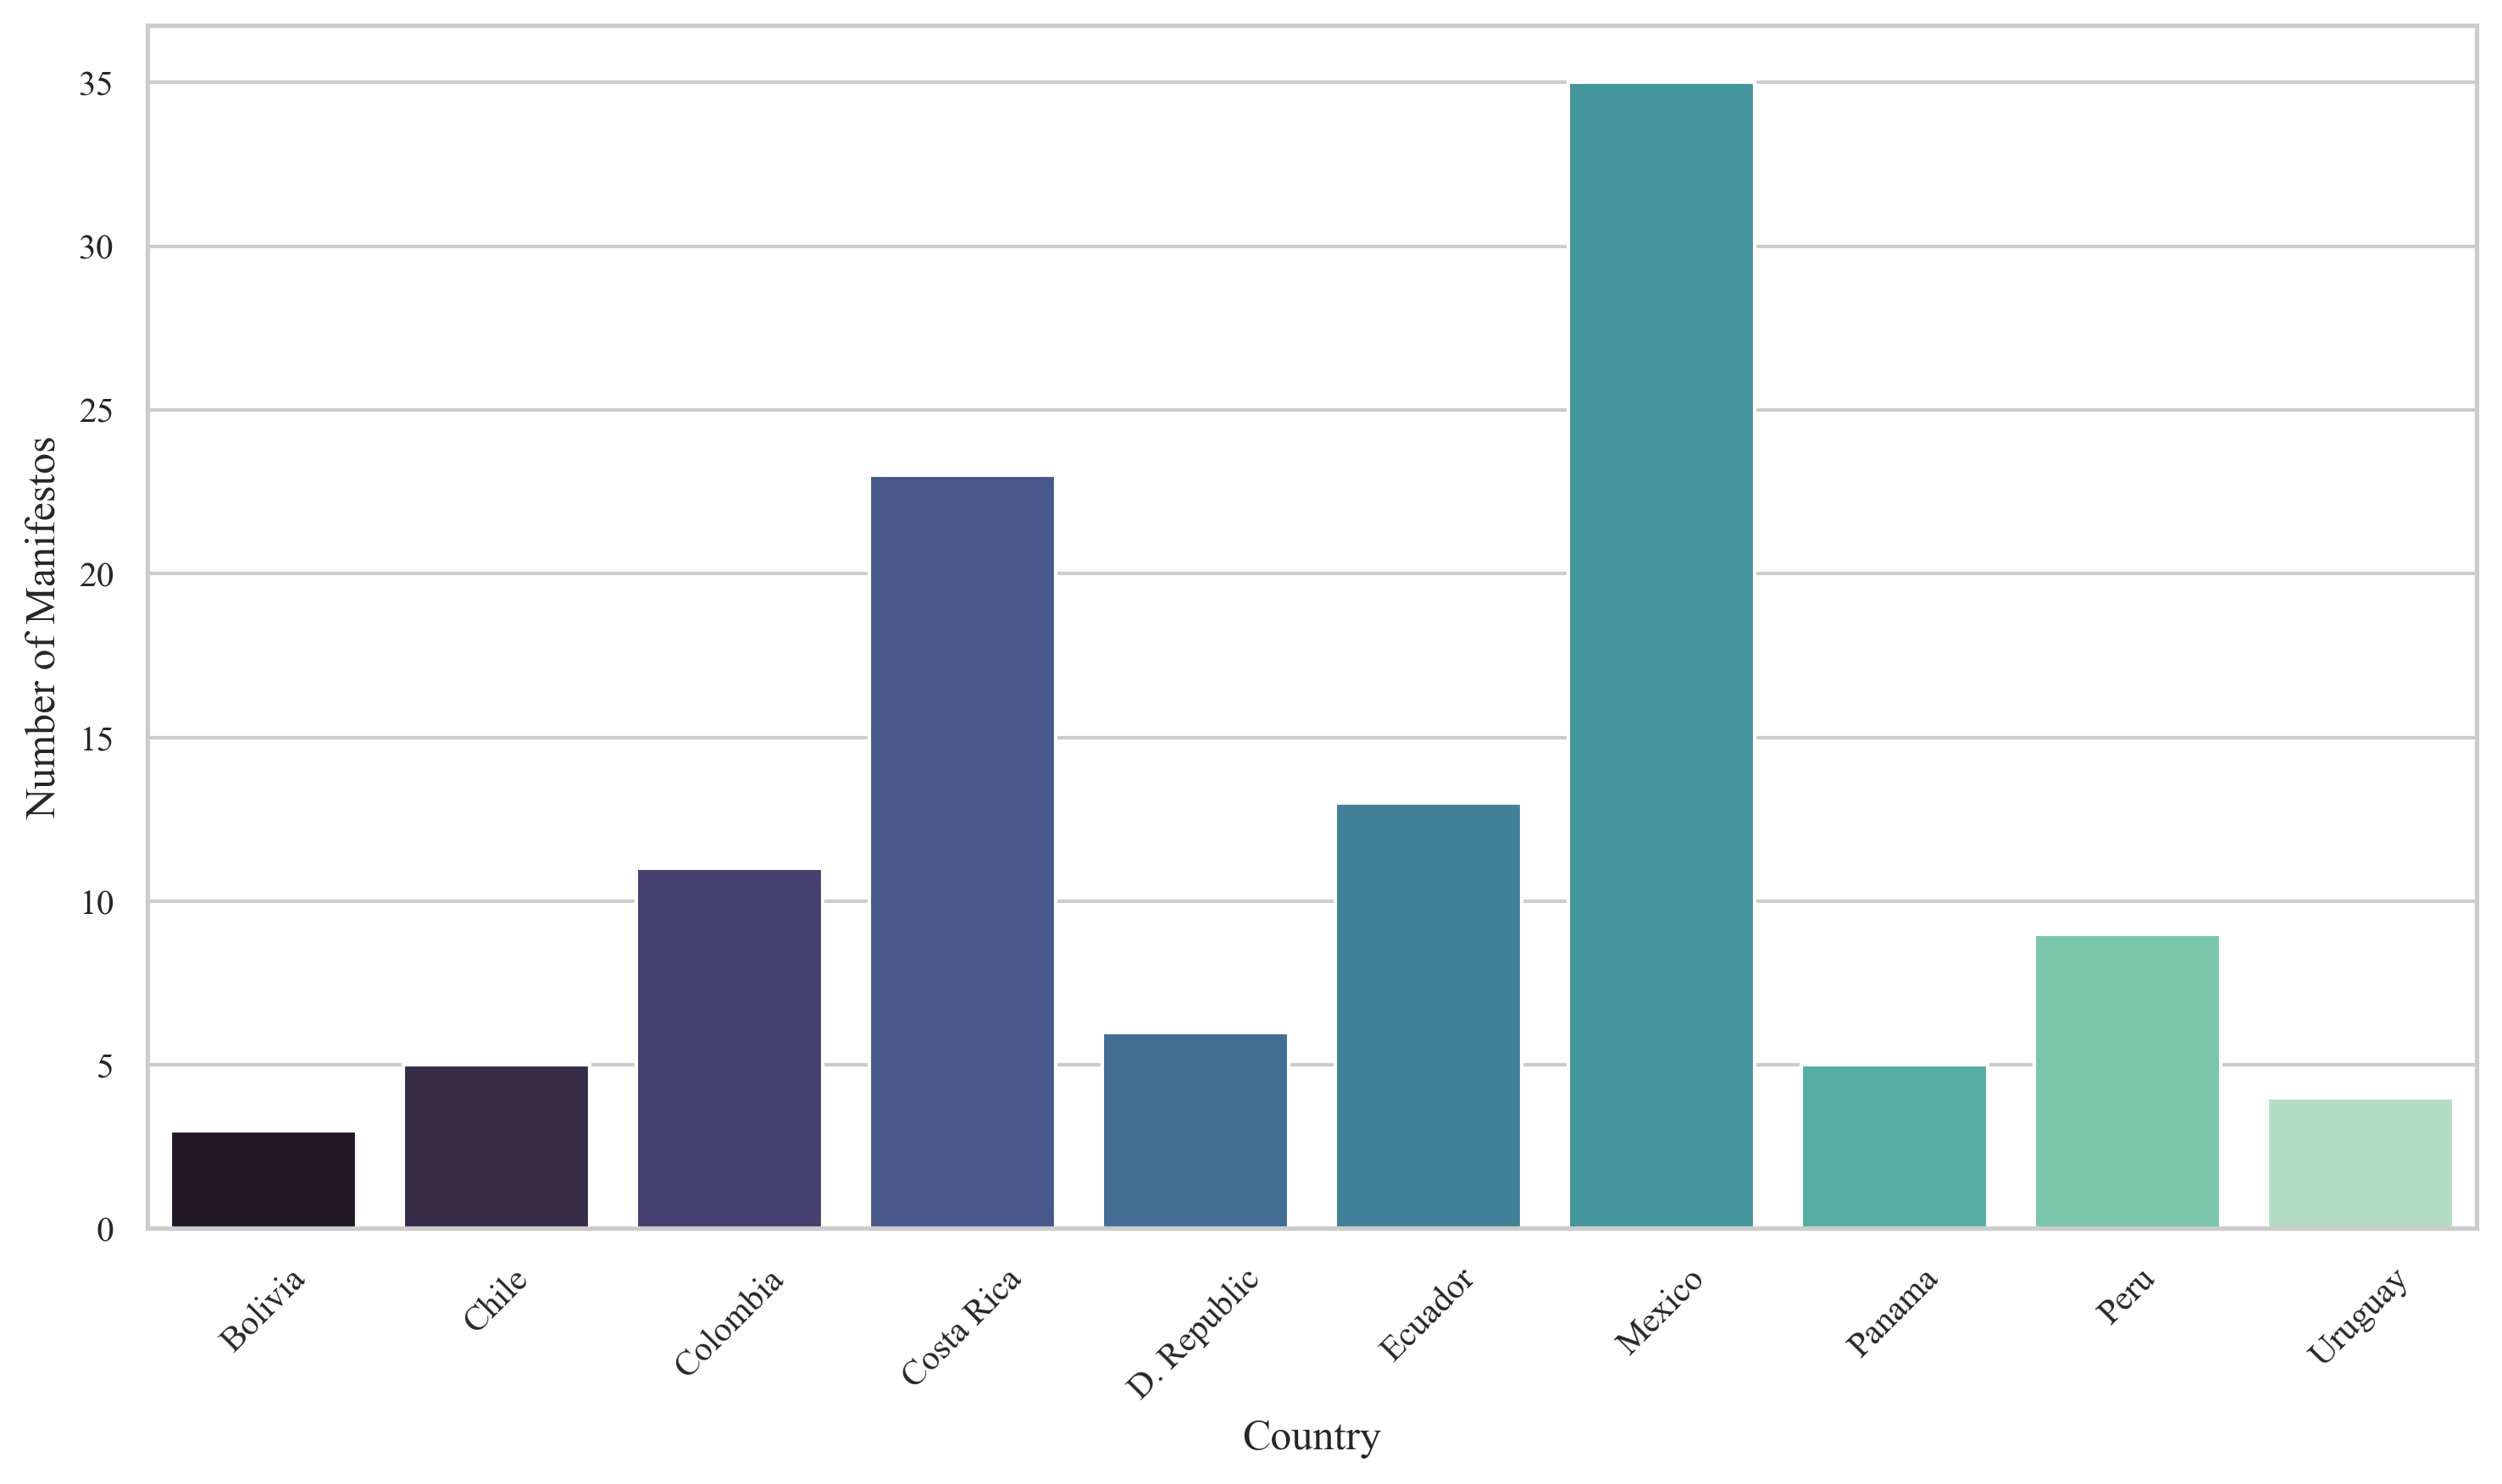
\includegraphics[width=0.8\textwidth]{/Users/sarabcidf/Desktop/ASDS/Dissertation/FinalScripts/SummaryStats/manif_by_country.png} 
\end{figure}

\begin{figure}[H]
	\centering
	\caption{Number of Parties by Populism Score}
	\label{fig:yourfigure}
	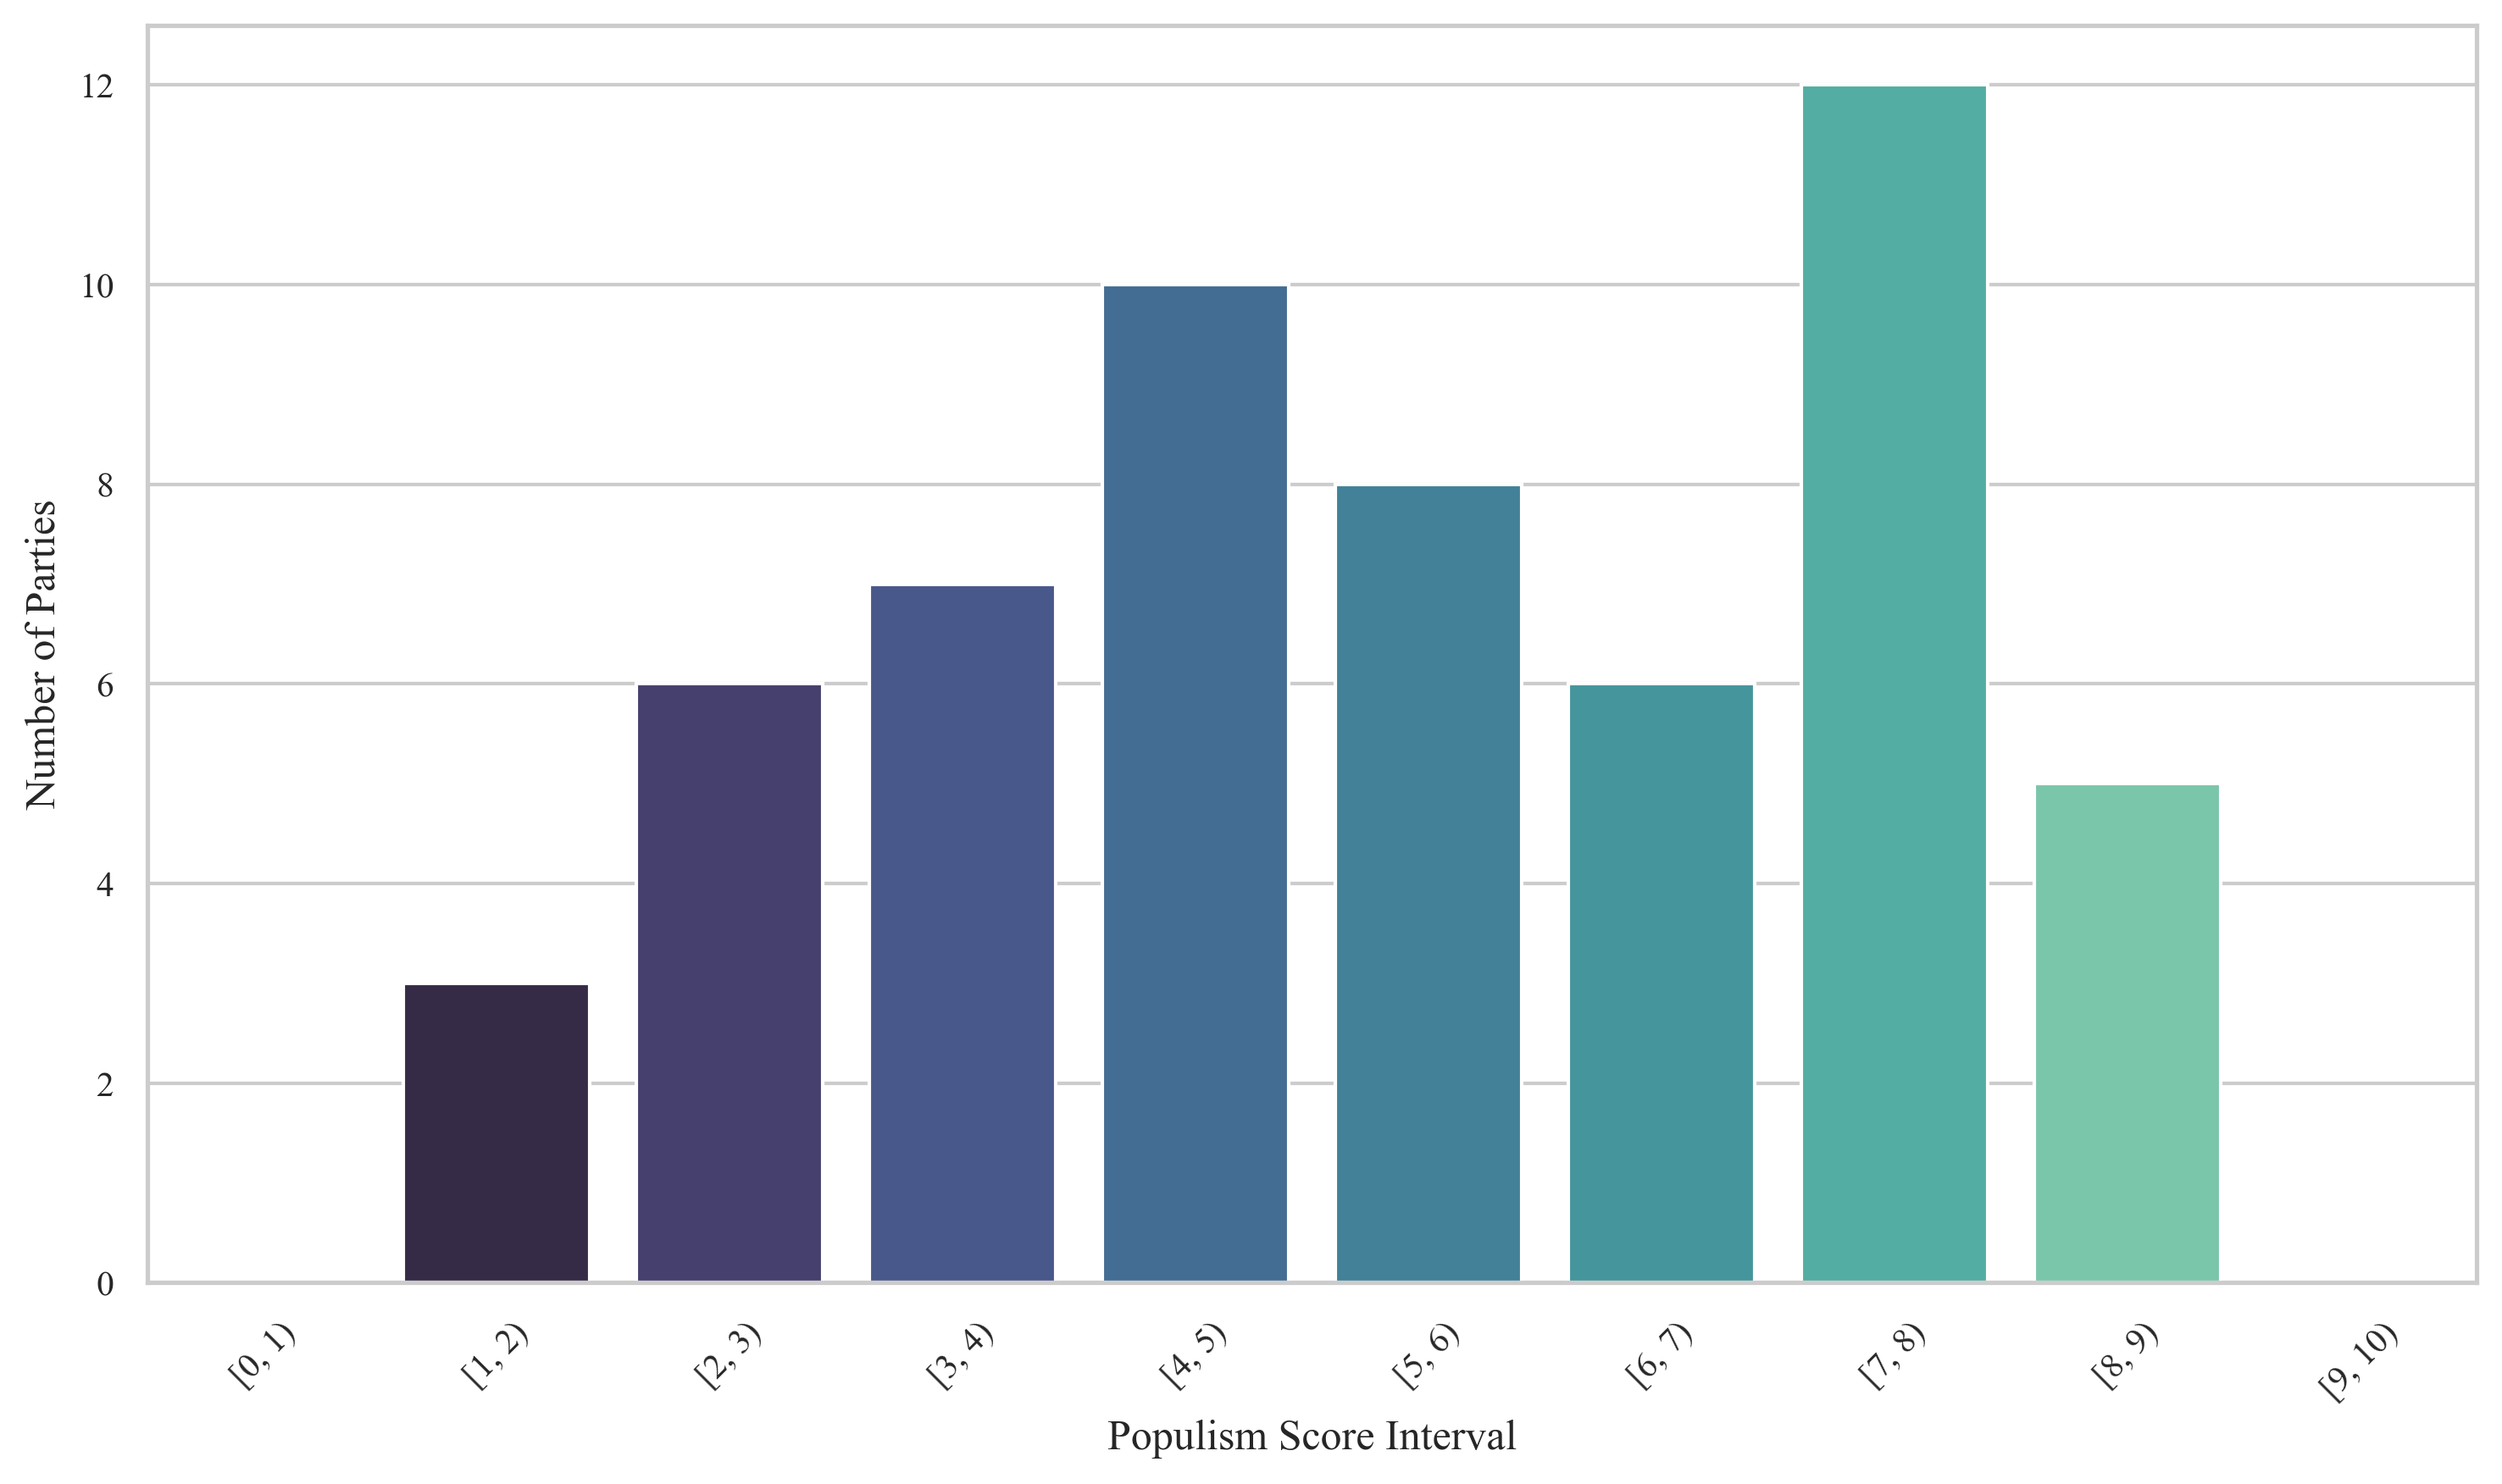
\includegraphics[width=0.8\textwidth]{/Users/sarabcidf/Desktop/ASDS/Dissertation/FinalScripts/SummaryStats/parties_by_pop_score.png} 
\end{figure}

\begin{figure}[H]
	\centering
	\caption{Number of Parties by Ideology (left-right)}
	\label{fig:yourfigure}
	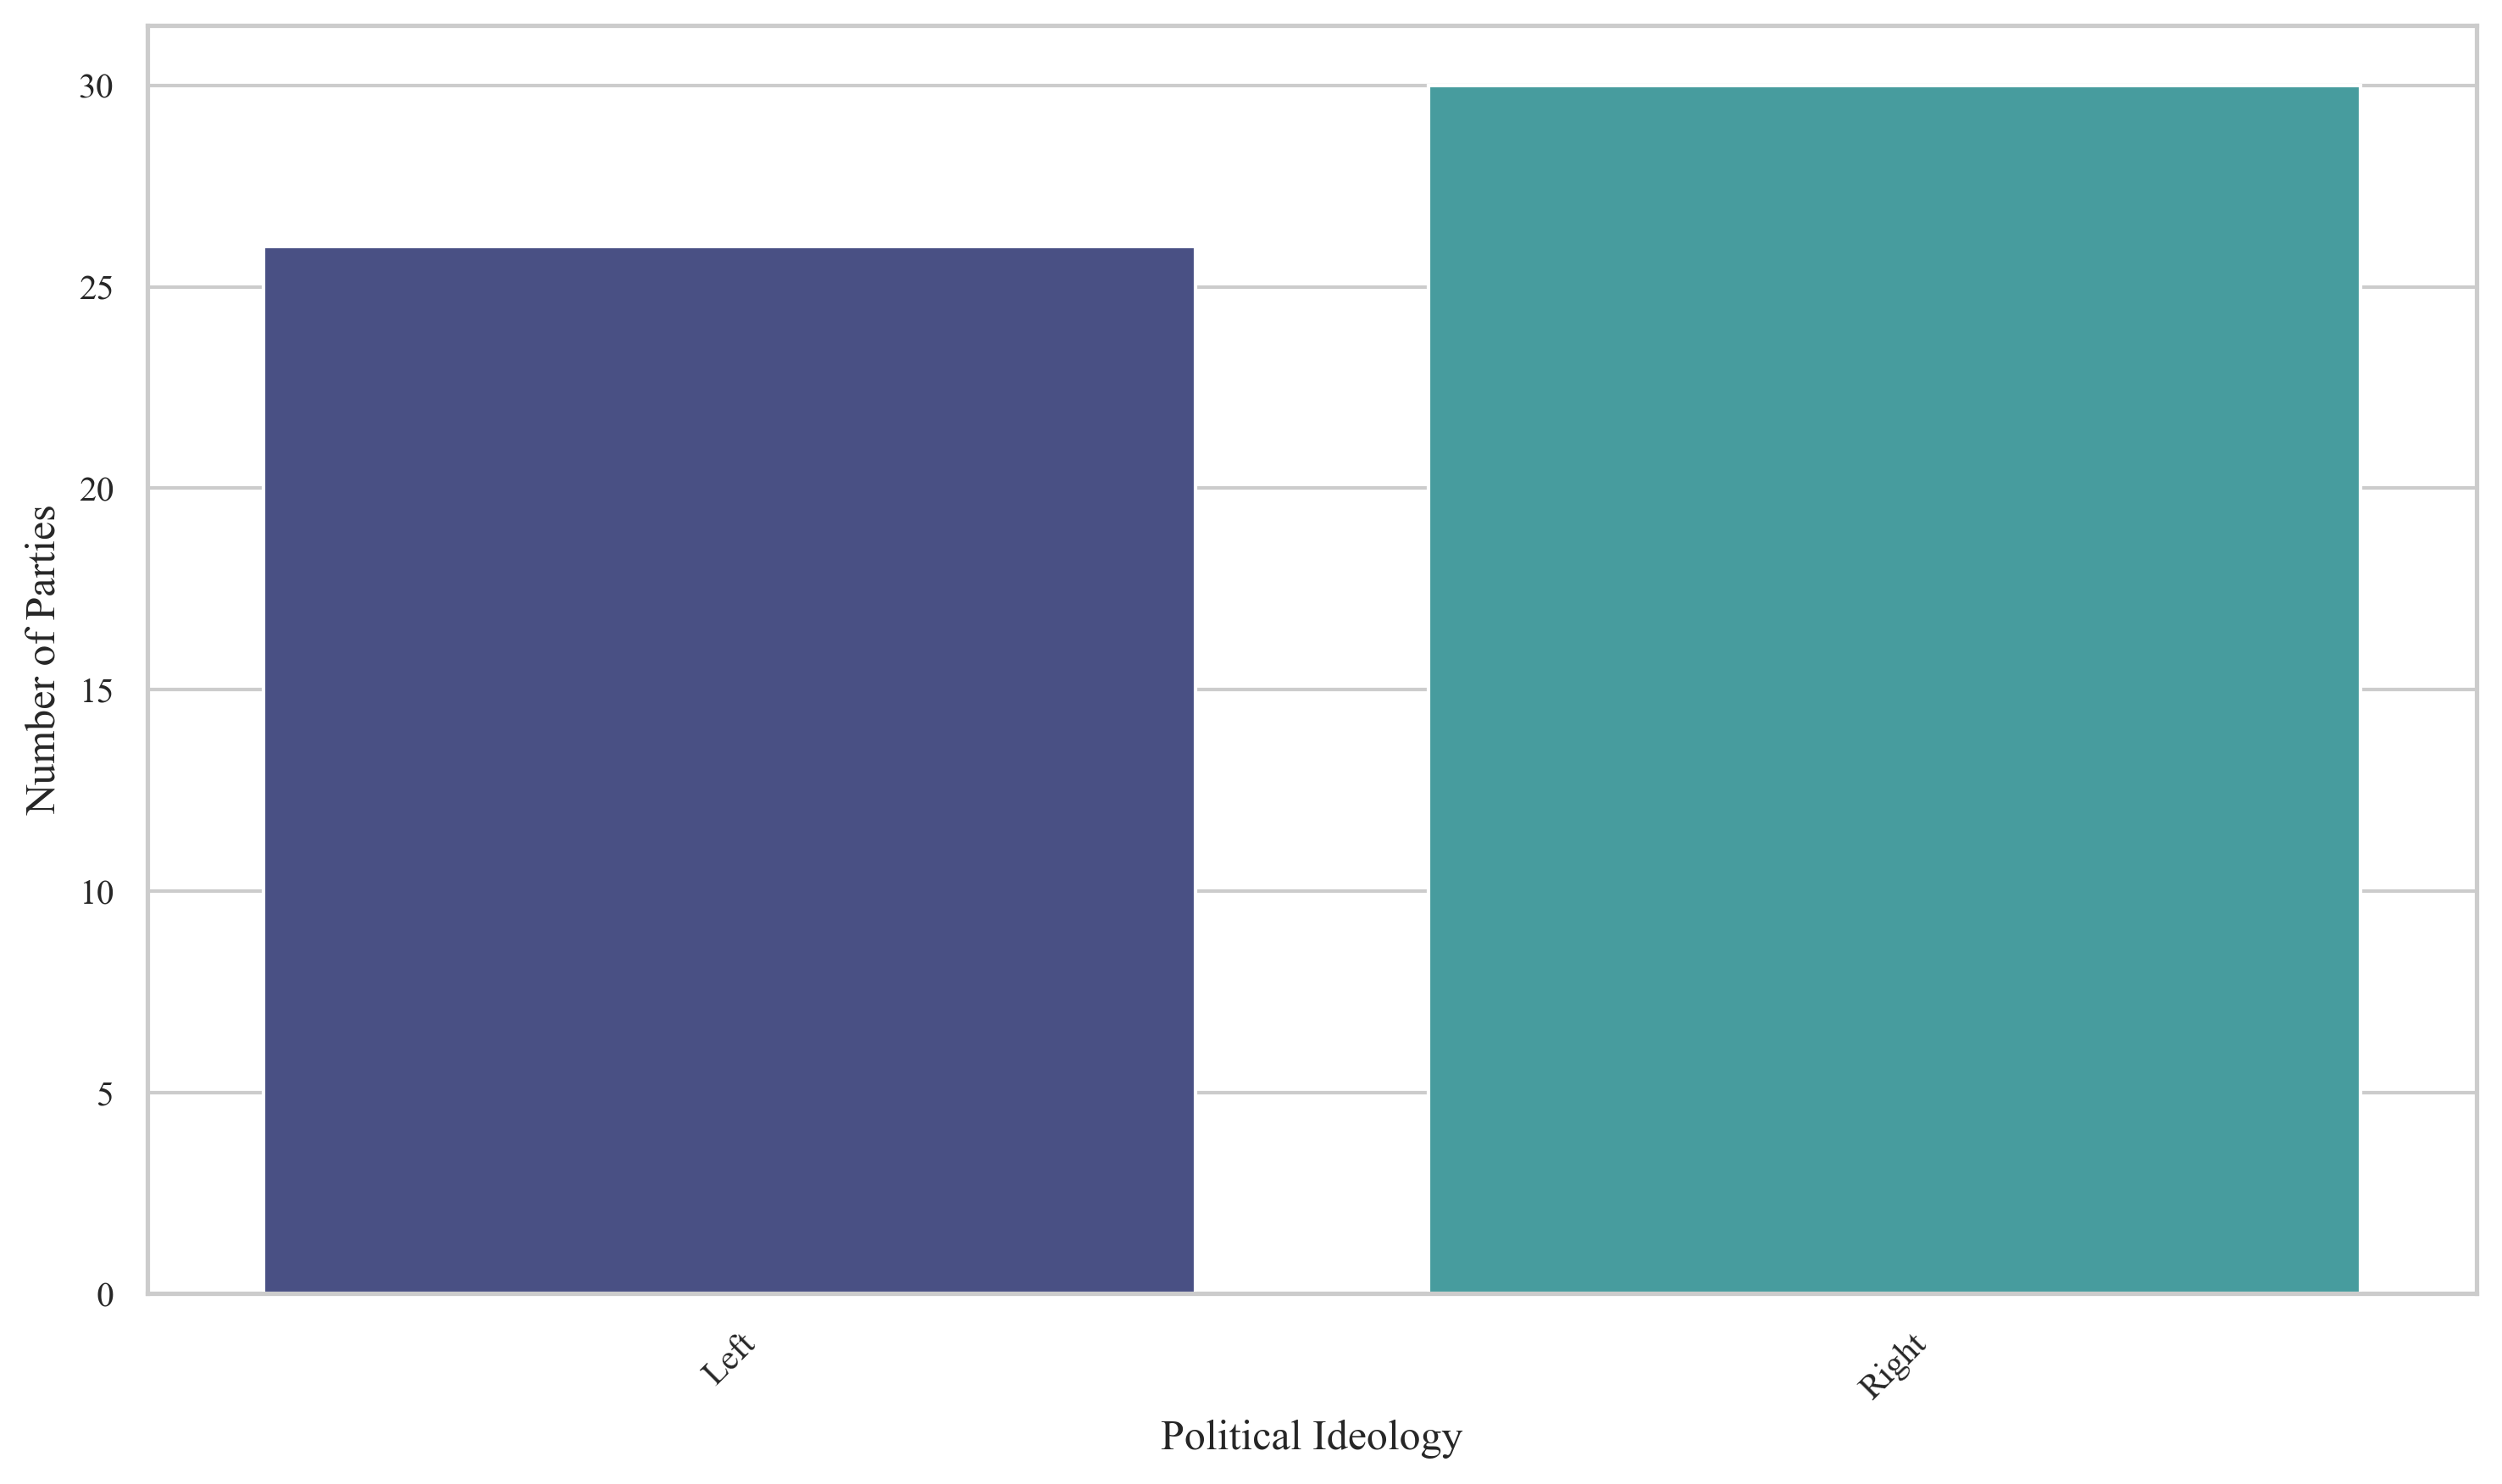
\includegraphics[width=0.8\textwidth]{/Users/sarabcidf/Desktop/ASDS/Dissertation/FinalScripts/SummaryStats/parties_by_ideology.png} 
\end{figure}

\noindent As it is shown above, some countries like Mexico or Costa Rica are over-represented in the dataset, in terms of the number of available manifestos. This over-representation comes from the fact that the MP has gathered a large number of manifestos from the two countries, as well from the losses that resulted when merging with the GPS. In other words, these countries are well covered in both sources. As expeccted, this over-representation also permeates to the sentence-level dataset, but the fact that the sample of sentences is unbalanced by country is not a source of concern. 

Moreover, while the distribution of parties by populism score looks more Normal, there is also a slight over-representation of significantly populist parties, scoring between 7-8 on average. The plot of parties per populism score also shows that there is considerable (and desierable) variation in the levels of levels of populism in the dataset. In addition, there are slightly more right-wing parties in the sample, although the number of parties is well balanced in this sense. 

\section{Results}

\vspace{.25cm}
\subsection{Model Results and Evaluation}

\vspace{.25cm}
\noindent Table 2 below presents key model performance scores and hyperparameters for the different country models. First, the table presents the MSE and the best score achieved for each model. Bolivia has the lowest values of both metrics, with an MSE of 0.163 and a best score of 1.17, while Costa Rica and Chile have the largest values, with over 3.1. The resulting optimal maximum depth, minimum samples per leaf, and number of estimators vary considerably by country, showing the data have different characteristics. 

For Bolivia, which shows the lowest MSE, the optimal hyperparameters were a maximum depth of 10, a minimum samples per leaf of 1, and 300 estimators, suggesting that a relatively deep and complex ensemble model was needed to pick up on the complexities in the data. For Costa Rica, on the other hand, a less constrained tree depth was more suitable, as the model does not specify a maximum depth, uses a minimum samples per leaf of 2, and employs 300 estimators. Other metrics such as error rates and learning curves can be consulted in Section 2 of the Online Appendix 2. 

\begin{table}[H]
	\centering
	\caption{Scores and Hyperparameters}
	\begin{tabular}{|l|r|r|r|r|r|}
		\hline
		\textbf{Country} & \textbf{MSE} & \textbf{Best Score} & \textbf{Max Depth} & \textbf{Min Samples Leaf} & \textbf{N Estimators} \\
		\hline
		Bolivia       &  0.163 &       0.170 &       10 &                 1 &           300 \\
		Colombia      &  2.673 &       2.638 &       10 &                 2 &           200 \\
		Costa Rica    &  3.190 &       3.315 &         None &                 2 &           300 \\
		Ecuador       &  1.706 &       1.866 &          None &                 2 &           300 \\
		Chile         &  3.365 &       3.366 &       10 &                 2 &           300 \\
		Panama        &  2.879 &       3.003 &          None &                 1 &           200 \\
		Uruguay       &  0.345 &       0.358 &          None &                 2 &           300 \\
		D. Republic   &  0.325 &       0.303 &       10 &                 2 &           100 \\
		Mexico        &  1.318 &       1.465 &          None &                 2 &           300 \\
		Peru          &  1.122 &       1.138 &          None &                 2 &           300 \\
		\hline
	\end{tabular}
\end{table}
	
\noindent The most relevant features for each model were explored as an evaluation/validation exercise. Table 3 below shows the three most relevant features by country, in Spanish as well as their translation to English, with relevant words highlighted in bold. For some countries, like Bolivia, Colimbia, Uruguay or the Dominican Republic, clearly people-centric words such as ``people", ``all", or ``citizen" are among the top features for predicting populism. Interestingly, the countries for which features like these are relevant are the same as the countries for which the model performed best in terms of MSE. The 10 most relevant features for each country can be consulted in Section 2 of the Online Appendix 2. 	
	
	\begin{table}[H]
		\centering
		\caption{Most Relevant Features by Country}
		\begin{tabular}{|l|l|l|}
			\hline
			\multicolumn{1}{|c|}{\textbf{Country}} & \multicolumn{1}{c|}{\textbf{Top Features}} & \multicolumn{1}{c|}{\textbf{Translation}} \\
			\hline
			Bolivia     & \textbf{gente}, \textbf{todos}, baterías          & \textbf{people}, \textbf{all}, batteries \\
			Colombia    & \textbf{sociedad}, \textbf{social}, \textbf{universal}     & \textbf{society}, \textbf{social}, \textbf{universal} \\
			Costa Rica  & restauración, paz, \textbf{ciudadana}    & restoration, peace, \textbf{citizen} \\
			Ecuador     & \textbf{ecuatorianos}, ecuador, desarrollo & \textbf{ecuatorians}, ecuador, development \\
			Chile       & chile, sistema, afrontar        & chile, system, face \\
			Panama      & ministerio, buscaremos, \textbf{pobres}  & ministry, seek, \textbf{poor} \\
			Uruguay     & \textbf{social}, \textbf{desarrollo}, estratégicas & \textbf{social}, \textbf{development}, strategic \\
			D. Republic & moderno, \textbf{gente}, \textbf{ciudadano}       & modern, \textbf{people}, \textbf{citizen} \\
			Mexico      & partido, \textbf{morena}, \textbf{neoliberal}     & party, \textbf{morena}, \textbf{neoliberal} \\
			Peru        & problema, estratégicas, lineamiento & problem, strategic, guideline \\
			\hline
		\end{tabular}
	\end{table}

\vspace{.25cm}
\subsection{Model Validation}

\vspace{.25cm}
\noindent Table 4 below presents a sample of (scaled) predictions at the party level, as a validation exercise. The sample was obtained by sorting the 55 parties in the dataset by their assigned scaled prediction, assigning them into 5 bins, and then randomly picking two parties per bin, looking at a total of 10 parties The aim of the exercise is to explore the populism scores the models assign to parties, and to see whether the result is expected. 

The scaled predictions range from 4.04 to 7.27, with the Movement towards Socialism from Bolivia having the highest score. This score is consistent with the party's well-known populist rhetoric and policies under the leadership of Evo Morales. On the lowest side of the spectrum is the Citizens' Movement from Mexico. This result is also consistent with the parties moderate stance. The predictions for all 55 parties can be consulted in section 2.11 of Online Appendix 2. 

\begin{table}[H]
	\centering
	\caption{Party Name, Country, and Scaled Prediction}
	\begin{tabular}{|>{\centering\arraybackslash}m{6cm}|>{\centering\arraybackslash}m{3cm}|>{\centering\arraybackslash}m{3cm}|}
		\hline
		\textbf{Party Name} & \textbf{Country} & \textbf{Scaled Prediction} \\ \hline
		\multicolumn{1}{|>{\raggedright\arraybackslash}m{6cm}|}{Movement towards Socialism - Political Instrument for the Sovereignty of the Peoples} & Bolivia & 7.27 \\ \hline
		\multicolumn{1}{|>{\raggedright\arraybackslash}m{6cm}|}{Proud and Sovereign Fatherland Alliance Movement} & Ecuador & 6.98 \\ \hline
		\multicolumn{1}{|>{\raggedright\arraybackslash}m{6cm}|}{National Solidarity Alliance} & Peru & 5.65 \\ \hline
		\multicolumn{1}{|>{\raggedright\arraybackslash}m{6cm}|}{Alliance for Progress of Peru} & Peru & 5.62 \\ \hline
		\multicolumn{1}{|>{\raggedright\arraybackslash}m{6cm}|}{Party of U} & Colombia & 5.36 \\ \hline
		\multicolumn{1}{|>{\raggedright\arraybackslash}m{6cm}|}{Alternative Democratic Pole} & Colombia & 5.26 \\ \hline
		\multicolumn{1}{|>{\raggedright\arraybackslash}m{6cm}|}{Progressive Movement} & Mexico & 4.51 \\ \hline
		\multicolumn{1}{|>{\raggedright\arraybackslash}m{6cm}|}{National Integration Party} & Costa Rica & 4.50 \\ \hline
		\multicolumn{1}{|>{\raggedright\arraybackslash}m{6cm}|}{Alliance for Mexico 2006} & Mexico & 4.18 \\ \hline
		\multicolumn{1}{|>{\raggedright\arraybackslash}m{6cm}|}{Citizens' Movement} & Mexico & 4.04 \\ \hline
	\end{tabular}
\end{table}

\noindent Additionally, an exploration of the scores assigned to a sample of sentences in the test data was also carried out. Table 5 below presents the scores that the regressor assigned to 10 sentences that were selected by sorting the test data, assigning observations into 5 bins, and randomly selecting two sentences per bin to get sentences belonging to the full spectrum. From this table, it can be observed that higher scores are given to sentences that contain people-centric features, even coinciding with features that came up among the most important ones. The first sentence in the table, for instance, scores 7.28 and contains the words ``Panamanian" and ``poor". The two bottom sentences, on the other hand, do not contain this sort of vocabulary, and consistently come from parties that are not considered populist. 

\begin{landscape}
	
	\begin{longtable}{|>{\centering\arraybackslash}m{7cm}|>{\centering\arraybackslash}m{7cm}|>{\centering\arraybackslash}m{2cm}|>{\centering\arraybackslash}m{2cm}|>{\centering\arraybackslash}m{2cm}|}
		\caption{Clean Sentence, Scaled Prediction, Party Name, Country, and Clean Sentence Translation} \\
		\hline
		\textbf{Clean Sentence} & \textbf{Clean Sentence Translation} & \textbf{Scaled Prediction} & \textbf{Party Name} & \textbf{Country} \\ \hline
		\endfirsthead
		
		\hline
		\textbf{Clean Sentence} & \textbf{Clean Sentence Translation} & \textbf{Scaled Prediction} & \textbf{Party Name} & \textbf{Country} \\ \hline
		\endhead
		
		\hline
		\endfoot
		
		\hline
		\endlastfoot
		
		% Adjust columns for vertical centering without horizontal centering
		\multicolumn{1}{|>{\raggedright\arraybackslash}m{7cm}|}{reduciremos impuestos obstáculos evitan disminuir costo vida \textbf{panameños} \textbf{pobres}} & \multicolumn{1}{|>{\raggedright\arraybackslash}m{7cm}|}{we will reduce taxes obstacles that prevent reducing the cost of living for poor \textbf{Panamanians}} & 7.28 & Democratic Change & Panama \\ \hline
		\multicolumn{1}{|>{\raggedright\arraybackslash}m{7cm}|}{construcciones infraestructura física \textbf{desarrollo} productivo convierten plataforma permitirá consolidar cambio económico estructural país} & \multicolumn{1}{|>{\raggedright\arraybackslash}m{7cm}|}{physical infrastructure constructions productive \textbf{development} become a platform that will consolidate the structural economic change of the country} & 6.94 & Proud and Sovereign Fatherland Alliance Movement & Ecuador \\ \hline
		\multicolumn{1}{|>{\raggedright\arraybackslash}m{7cm}|}{dimensión compromiso descentralización fomentar \textbf{cooperativas} empresas energéticas regionales foco \textbf{desarrollo} económico local} & \multicolumn{1}{|>{\raggedright\arraybackslash}m{7cm}|}{dimension of commitment to decentralization to promote \textbf{cooperatives} of regional energy companies focus on local economic \textbf{development}} & 5.58 & Approve Dignity & Chile \\ \hline
		\multicolumn{1}{|>{\raggedright\arraybackslash}m{7cm}|}{considerará vulnerabilidad riesgos \textbf{comunidades} incorporando principios prevención responsabilidad materia} & \multicolumn{1}{|>{\raggedright\arraybackslash}m{7cm}|}{will consider the vulnerability and risks of \textbf{communities} incorporating principles of prevention and responsibility in the matter} & 5.55 & Broad Front & Chile \\ \hline
		\multicolumn{1}{|>{\raggedright\arraybackslash}m{7cm}|}{propulsar negocios extraer} & \multicolumn{1}{|>{\raggedright\arraybackslash}m{7cm}|}{boost extractive businesses} & 5.46 & Alliance Possible Peru & Peru \\ \hline
		\multicolumn{1}{|>{\raggedright\arraybackslash}m{7cm}|}{ecoturismo \textbf{subdesarrollado} perú inmensas áreas naturales aprovechables propósitos \textbf{desarrollar} turismo sostenible} & \multicolumn{1}{|>{\raggedright\arraybackslash}m{7cm}|}{underdeveloped ecotourism in Peru, immense natural areas exploitable for purposes of \textbf{developing} sustainable tourism} & 5.02 & Alliance for Progress of Peru & Peru \\ \hline
		\multicolumn{1}{|>{\raggedright\arraybackslash}m{7cm}|}{gobierno federal cumpla satisfaga demandas \textbf{sociales}} & \multicolumn{1}{|>{\raggedright\arraybackslash}m{7cm}|}{federal government fulfills and satisfies \textbf{social} demands} & 4.51 & Labor Party & Mexico \\ \hline
		\multicolumn{1}{|>{\raggedright\arraybackslash}m{7cm}|}{proponemos frente \textbf{común} gobierno federal gobiernos ayuntamientos combate inseguridad reforzando programas conjuntos promoviendo reformas legislativas acelerando transformación estructuras administrativas operativas necesarias modernización depuración profesionalización sistemas seguridad \textbf{justicia} municipios país} & \multicolumn{1}{|>{\raggedright\arraybackslash}m{7cm}|}{we propose a \textbf{common} front between the federal government, local governments, and municipalities to combat insecurity by strengthening joint programs, promoting legislative reforms, and accelerating the transformation of necessary administrative and operational structures for the modernization, purification, and professionalization of security and \textbf{justice} systems in the country's municipalities} & 3.81 & Commitment for Mexico & Mexico \\ \hline
		\multicolumn{1}{|>{\raggedright\arraybackslash}m{7cm}|}{fortalecimiento institucionalidad \textbf{igualdad} equidad género} & \multicolumn{1}{|>{\raggedright\arraybackslash}m{7cm}|}{strengthening institutional \textbf{equality} and gender equity} & 3.16 & Citizen’s Action Party & Costa Rica \\ \hline
		\multicolumn{1}{|>{\raggedright\arraybackslash}m{7cm}|}{siguientes etapas conducirán formación visión estratégica nacional} & \multicolumn{1}{|>{\raggedright\arraybackslash}m{7cm}|}{the following stages will lead to the formation of a national strategic vision} & 2.24 & Broad Front & Uruguay \\ \hline
	\end{longtable}
	
\end{landscape}

\vspace{.25cm}
\subsection{Results of the Application}

\vspace{.25cm}
\noindent In order to examine the relationship between the anti-elitist and people-centric components, and populism levels in Latin America and Europe, this study used the GPS questions described in Section 4.2.2. All the variables capturing the dimensions of populism (``Corrupt Politicians", ``People Should Decide", ``Strongman Rule" and ``Will of the People) were used as independent variables in four different models. All specifications also included an indicator Region variable on its own (where the region can be either Europe or Latin America), and in an interaction with each of the dimensions of populism, and the ideology variable (also the average expert score, where 0 is perfectly left-leaning and 10 is perfectly right-leaning) as a control. 

Ultimately, the goal is to evaluate whether the association (its sign and magnitude) between each of these dimensions and the level of populism varies according to the region. While the GPS offers no measures of the levels of anti-elitism or people-centrism associated to political parties, this study assumes that the ``corrupt politicians" variable offered by the GPS would capture a similar dimension to anti-elitism, while the ``people should decide" and ``will of the people" variables should be indicative of people-centric tendencies. The results of running the three regressions are presented in Table 6. 

First, the estimated coefficient of the Ideology variable is close to zero in magnitude across all models, and it is only statistically significant (at the 95\% confidence level) in the Strongman Rule model, where it is -0.0802. This indicates that a one-unit increase in the Ideology scale (moving one point from more left-leaning to more right-leaning on the 10-point scale) is associated with a decrease of 0.08 units in the Populist Rhetoric scale, on average, while controlling for the Strongman Rule and Region variables.

Next, the Region variable shows varying effects across the models, indicating that the influence of being in Latin America versus Europe (the reference category) on populist rhetoric depends on the specific political dimension being considered. In the first model, being in Latin America is associated with a substantial increase in Populist Rhetoric (coefficient of 2.8990). However, in the second and fourth models, being in Latin America is associated with decreases in Populist Rhetoric (coefficients of -1.8812 and -3.2293, respectively). The third model shows a moderate positive effect (coefficient of 0.4129). These variations suggest that the context of Latin America either increases or decreases populist rhetoric depending on the particular dimension under examination.

For the first model, the estimated coefficient of Corrupt Politicians is 0.6536, and it is statistically significant to the 99\% confidence level. Thus, a one-unit increase in this scale is associated with a 0.6536 unit increase in Populist Rhetoric, on average, while controlling for the Ideology variable. While the effect of Corrupt Politicians on populist rhetoric is 0.6536 in Europe, the estimate for the coefficient of the interaction term suggests that, in Latin America, this effect decreases by 0.5806 units, resulting in an effect of 0.0730 on average. Therefore, on average, in Latin America, a one-unit increase in the perception of corrupt politicians is associated with a 0.073 unit increase in populist rhetoric, while controlling for the rest of the independent variables in the model. This finding is relevant, as it indicates that the association between the Corrupt Politicians and the Populist Rhetoric variables is considerably smaller for Latin America, compared to Europe.

From the second model, it is observable that a one-unit increase in the saliency of the People Should Decide variable is associated with a 0.1352 unit decrease in Populist Rhetoric, on average, while controlling for the Ideology variable. The interaction term between People Should Decide and Region is positive and statistically significant at the 99\% confidence level, with an estimated coefficient of 0.3869. Therefore, the association of the People Should Decide and the Populist Rhetoric variables that is observed in Europe is larger in Latin America. Specifically, in Latin America, the coefficient of the People Should Decide increases by 0.3869 units, resulting in a positive coefficient of magnitude 0.2517. While in Europe, the People Should Decide dimension is associated with a slight decrease in Populist Rhetoric, in Latin America, it is associated with an increase in the outcome, on average, while controlling for the rest of the independent variables in the model.

In the third model, the estimated coefficient for the Strongman Rule variable is 0.7419, and it is statistically significant at the 99\% confidence level. This indicates that a one-unit increase in the Strongman Rule variable is associated with a 0.7419 unit increase in Populist Rhetoric, on average, while controlling for the Ideology variable. The interaction term between Strongman Rule and Region has an estimated coefficient of -0.1329, which is not statistically significant. This suggests that the effect of the Strongman Rule variable on populist rhetoric does not significantly differ between Europe and Latin America. As a result, the overall effect of Strongman Rule on populist rhetoric remains positive in both regions, though slightly less so in Latin America (0.6090) compared to Europe (0.7419), on average.

Finally, in the fourth model, the estimated coefficient for the Will of the People variable is -0.5908, which is statistically significant at the 99\% confidence level. This indicates that a one-unit increase in the Will of the People scale is associated with a 0.5908 unit decrease in Populist Rhetoric, on average, while controlling for the Ideology variable. The interaction term between Will of the People and Region is positive and statistically significant at the 99\% confidence level, with an estimated coefficient of 0.7627. This means that while the Will of the People variable is associated with a decrease in Populist Rhetoric in Europe (-0.5908), in Latin America, this effect is reversed. In Latin America, the effect of the Will of the People variable on Populist Rhetoric increases by 0.7627 units, resulting in a positive effect of 0.1719 units, on average. Therefore, contrary to the negative association observed in Europe, the Will of the People dimension is associated with a slight increase in Populist Rhetoric in Latin America, on average, while controlling for the rest of the independent variables in the model.

\begin{landscape}

\begin{table}[H] 
	\centering
	\caption{Regression Results with Interaction Terms}
	\resizebox{1.2\textwidth}{!}{  % Adjust the scaling factor as needed
		\begin{tabular}{@{\extracolsep{2pt}}l@{\hspace{-15pt}}c@{\hspace{-15pt}}c@{\hspace{-15pt}}c@{\hspace{-15pt}}c}
			\hline
			\hline
			\\[-1.5ex]
			& \multicolumn{4}{c}{\textit{Dependent variable: Populist Rhetoric}} \\
			\cline{2-5}
			\\[-1.5ex]
			& \makecell{Corrupt \\ Politicians} & \makecell{People \\ Should Decide} & \makecell{Strongman \\ Rule} & \makecell{Will of the \\ People}  \\
			\hline
			\\[-1.5ex]
			Intercept & 2.1110\textsuperscript{***} & 6.5157\textsuperscript{***} & 2.9215\textsuperscript{***} & 7.9661\textsuperscript{***} \\
			& (0.3494) & (0.3859) & (0.2853) & (0.3832) \\
			Corrupt Politicians & 0.6536\textsuperscript{***} & & & \\
			& (0.0465) & & & \\
			Corrupt Politicians:Region [LatAm] & -0.5806\textsuperscript{***} & & & \\
			& (0.0935) & & & \\
			Ideology & 0.0212 & -0.0782 & -0.0802\textsuperscript{**} & 0.0111 \\
			& (0.0426) & (0.0540) & (0.0392) & (0.0491) \\
			People Should Decide & & -0.1352\textsuperscript{*} & & \\
			& & (0.0698) & & \\
			People Should Decide:Region [LatAm] & & 0.3869\textsuperscript{***} & & \\
			& & (0.1171) & & \\
			Region [LatAm] & 2.8990\textsuperscript{***} & -1.8812\textsuperscript{***} & 0.4129 & -3.2293\textsuperscript{***} \\
			& (0.5925) & (0.6564) & (0.4025) & (0.5979) \\
			Strongman Rule & & & 0.7419\textsuperscript{***} & \\
			& & & (0.0482) & \\
			Strongman Rule:Region [LatAm] & & & -0.1329 & \\
			& & & (0.0829) & \\
			Will of the People & & & & -0.5908\textsuperscript{***} \\
			& & & & (0.0744) \\
			Will of the People:Region [LatAm] & & & & 0.7627\textsuperscript{***} \\
			& & & & (0.1207) \\
			\hline
			\\[-1.5ex]
			Observations & 452 & 451 & 454 & 453 \\
			$R^2$ & 0.3097 & 0.0270 & 0.4155 & 0.1317 \\
			Adjusted $R^2$ & 0.3035 & 0.0183 & 0.4103 & 0.1239 \\
			Residual Std. Error & 2.0640 (df = 447) & 2.4291 (df = 446) & 1.8992 (df = 449) & 2.3199 (df = 448) \\
			F Statistic & 50.1263\textsuperscript{***} (df = 4; 447) & 3.0943\textsuperscript{**} (df = 4; 446) & 79.8028\textsuperscript{***} (df = 4; 449) & 16.9812\textsuperscript{***} (df = 4; 448) \\
			\\[-1.5ex]
			\hline
			\hline
			\\[-1.5ex]
			\textit{Note:} & \multicolumn{4}{r}{\textsuperscript{*}p$<$0.1; \textsuperscript{**}p$<$0.05; \textsuperscript{***}p$<$0.01} \\
		\end{tabular}
	}
\end{table}

\end{landscape}

\noindent From the above, it is relevant to note that, when comparing the effects of the different dimensions on the level of populism in Europe versus Latin America, the influence of Corrupt Politicians is substantially reduced, while the People Should Decide variable has a stronger positive effect on Populist Rhetoric, and the Will of the People variable shifts from having a negative effect to a slightly positive one on Populist Rhetoric. The relationship that the Corrupt Politicians and the People Should Decide variables have with the level of Populist Rhetoric is further examined and illustrated by Figures 4 and 5 below. 

The first scatterplot illustrates the relationship between Corrupt Politicians and the level of Populist Rhetoric. For Europe, a clear pattern emerges, where a positive association between both variables is visible. Moreover, as shown in the legend, the estimated coefficient of Corrupt Politicians in a bivariate regression with Populist Rhetoric (also visible on the plot) is 0.59, and is statistically significant to the 95\% confidence level. For Latin America, the scatterplot shows no clear pattern, and the coefficient of Corrupt Politicians in the biariate regression with Populist Rhetoric is estimated at 0.11, although it is not statistically significant. 

The second scatterplot illustrates the relationship between People Should Decide and Populist Rhetoric. While the patterns the plot reveals are less clear than in the first figure, the estimated slope of the regression lines are statistically significant, and suggest that the relationship between People Should Decide and Populism is negative in the case of Europe, with an estimate of -0.53 that is significant to the 95\% confidence level, while this relationship is positive in Latin America, with an estimated slope of 0.18 that is significant to the 90\% level. Additional scatterplots showing the relationship between the GPS populism dimensions variables and the level of populist rhetoric can be consulted in Online Appendix 3. 

These regression exercises provide evidence that the Corrupt Politicians variable, which is proxy for the anti-elitism dimension is less related to levels of populism in Latin America compared to Europe, while the People Should Decide and Will of the People variables, which are proxies for people-centrism, are more relevant in the Latin American context. Thus, these results support the studies hypotheses that the defining features of populism may vary (or at least vary in relevance) between the two regions, with stronger evidence in favor of a less pronounce association between anti-elitism and populism in Latin America compared to Europe, as the study hypothesized. 

\begin{landscape}

\begin{figure}[H]
	\vspace{1.5cm}
	\centering
	\caption{Corrupt Politicians Dimension vs. Populist Rhetoric in Latin American and European Parties}
	\label{fig:yourfigure}
	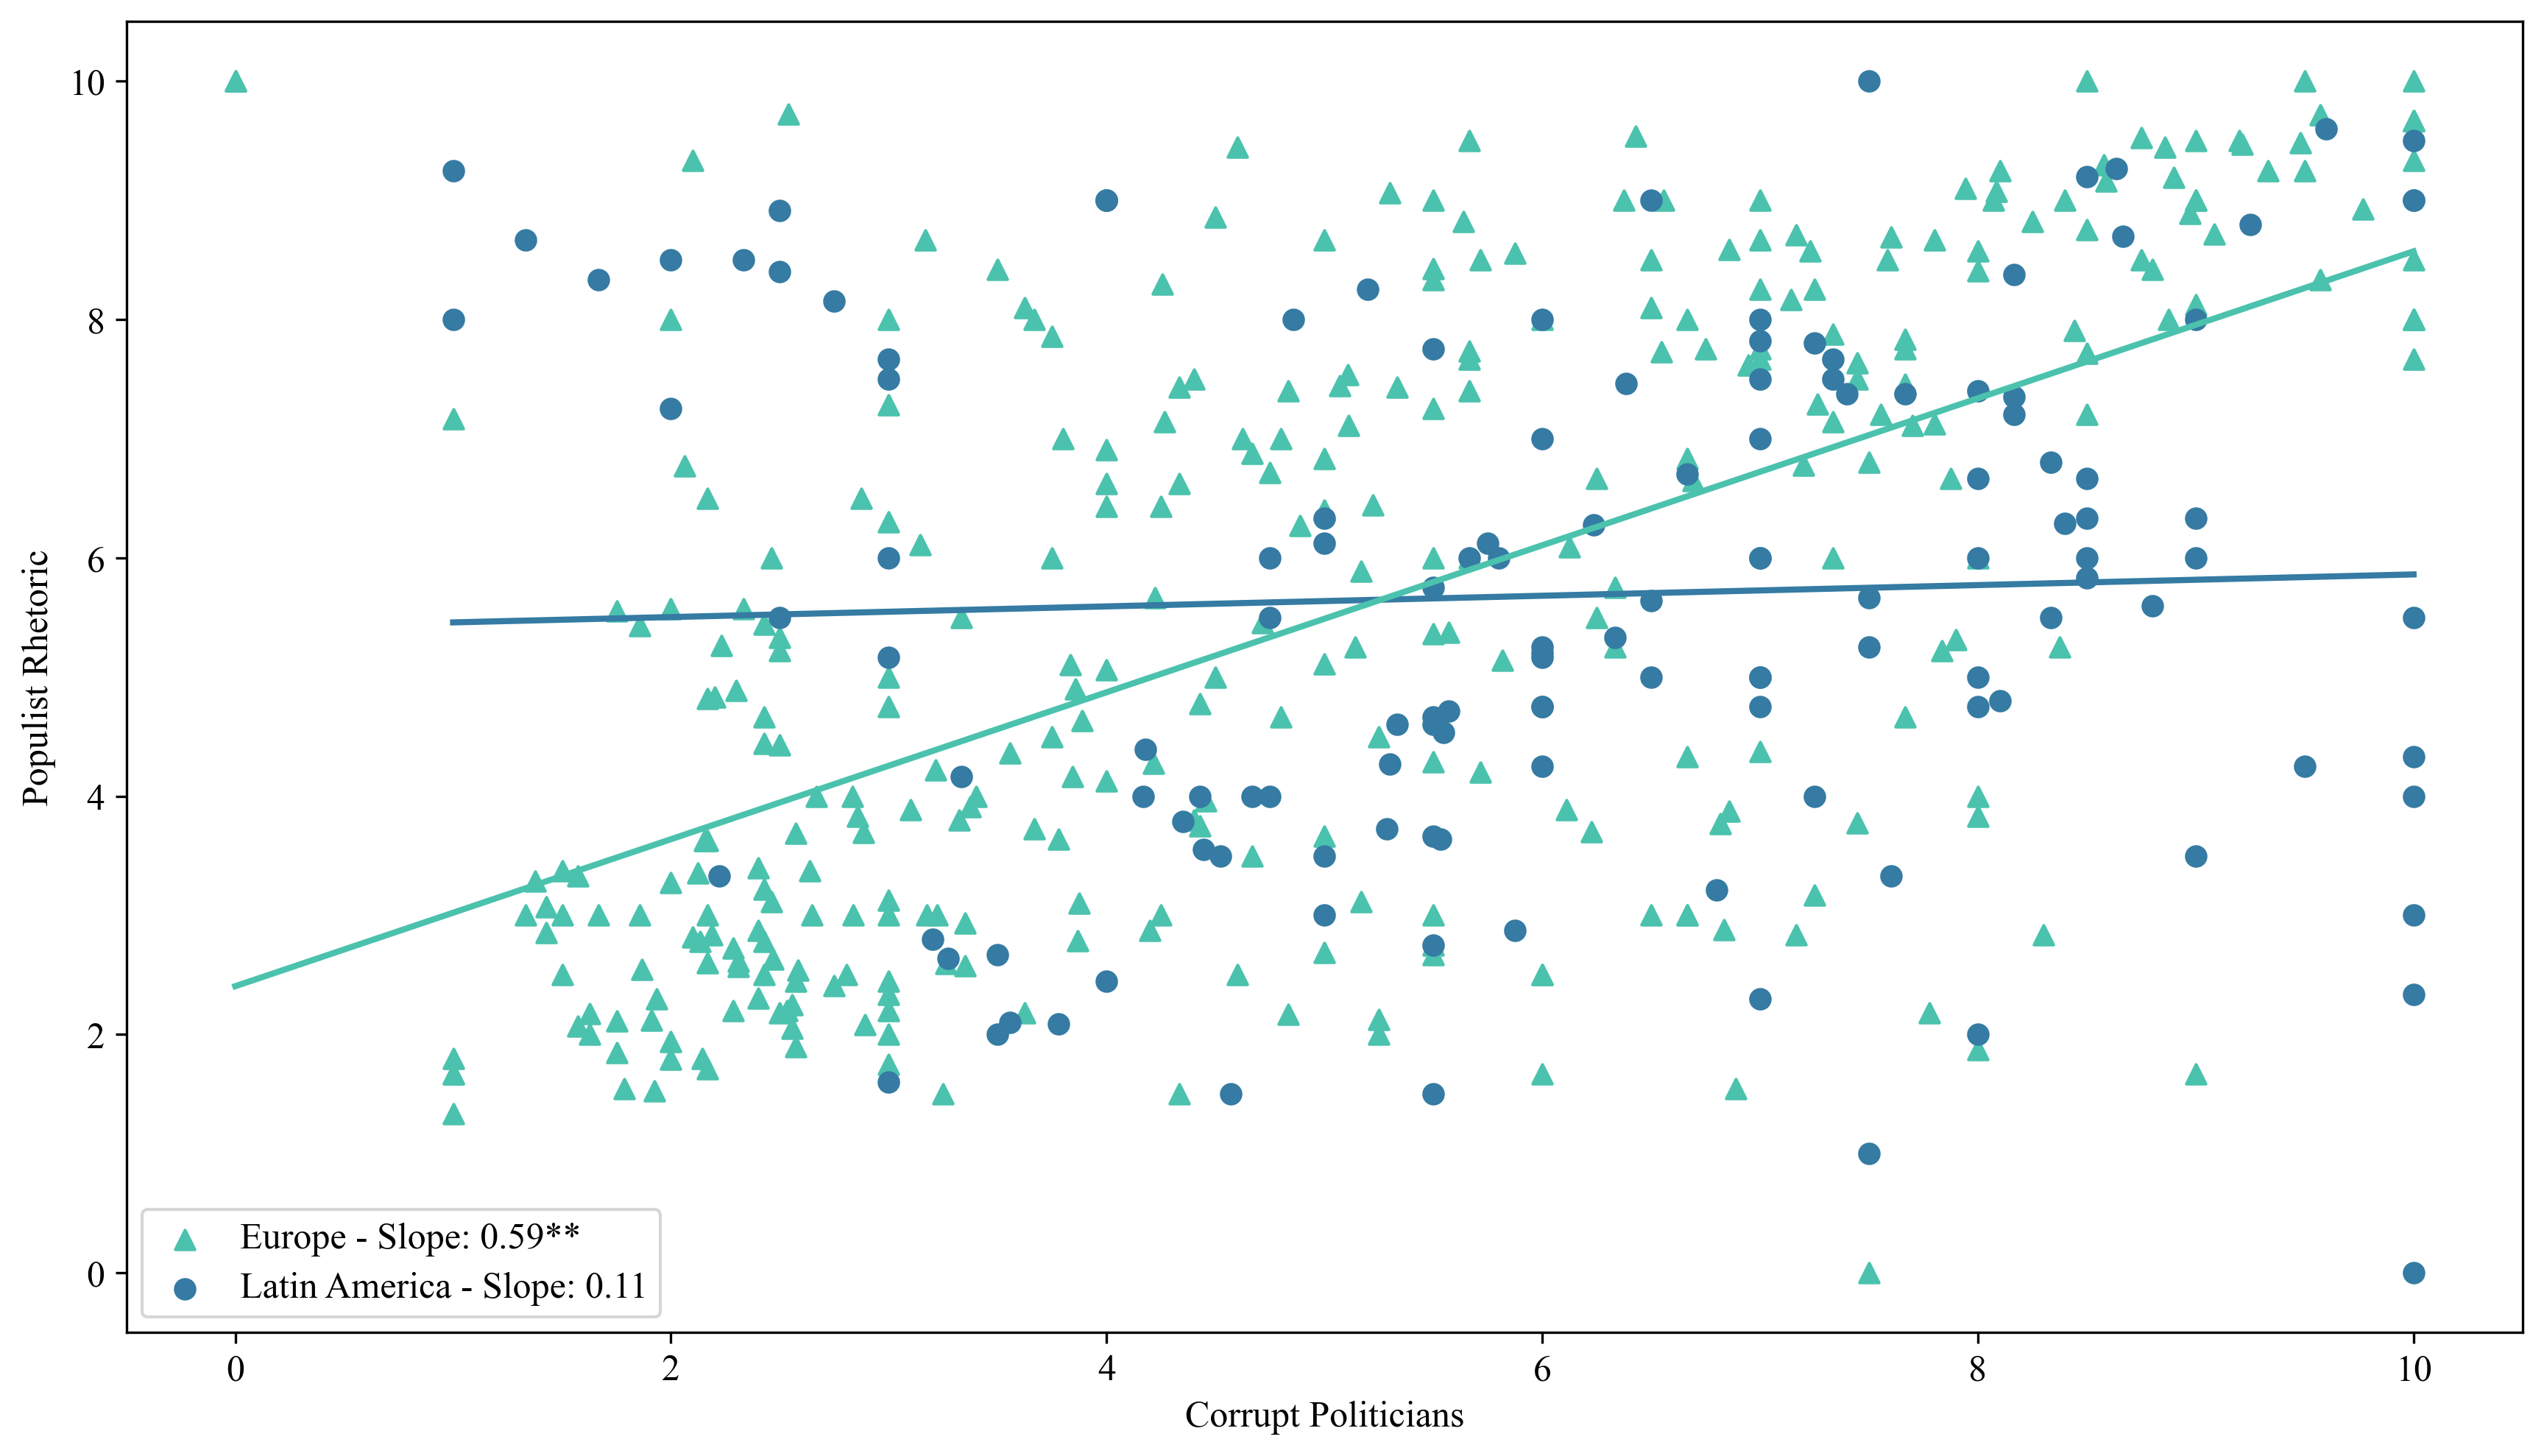
\includegraphics[width=1.3\textwidth]{/Users/sarabcidf/Desktop/ASDS/Dissertation/FinalScripts/CorRegAnalysis/corrupt_politicians_vs_populist_rhetoric_wide.png} 
\end{figure}

\begin{figure}[H]
	\vspace{1.5cm}
	\centering
	\caption{People Should Decide vs. Populist Rhetoric in Latin American and European Parties}
	\label{fig:yourfigure}
	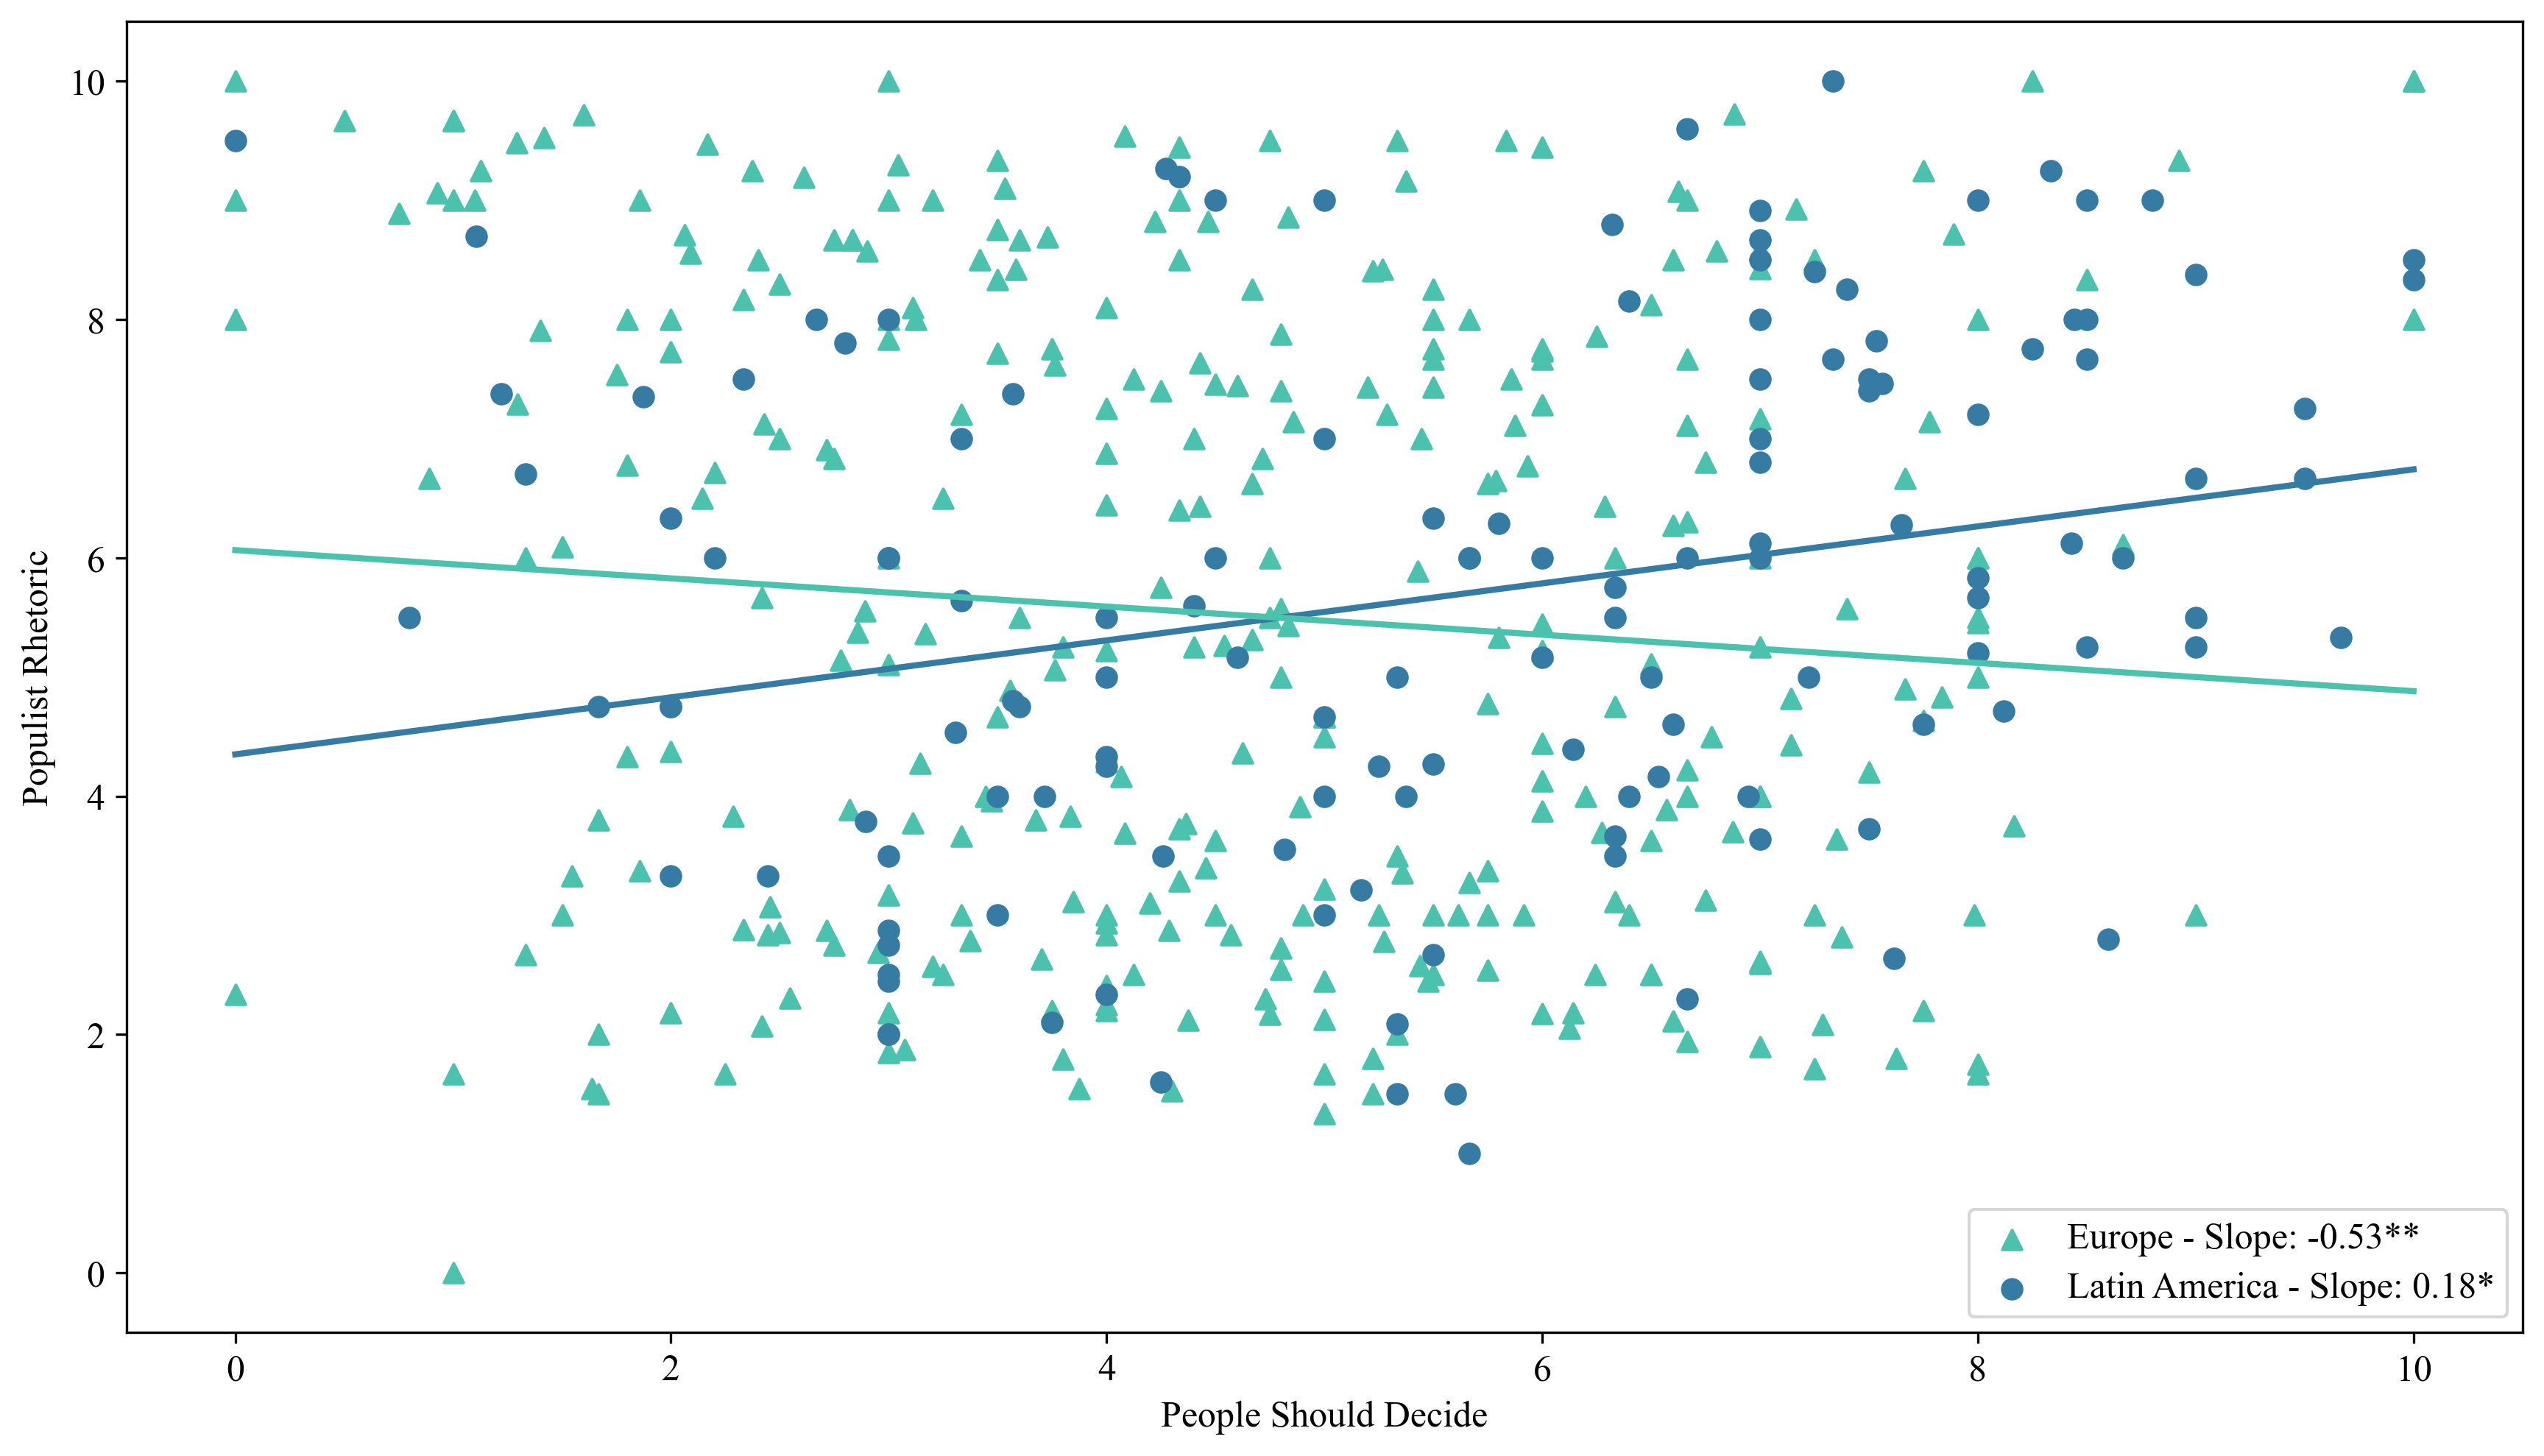
\includegraphics[width=1.3\textwidth]{/Users/sarabcidf/Desktop/ASDS/Dissertation/FinalScripts/CorRegAnalysis/people_should_decide_vs_populist_rhetoric_wide.png} 
\end{figure}

\end{landscape}

\section{Discussion and Conclusions} 

\vspace{.25cm}
\noindent This study introduces a new computational approach to measuring populism, addressing the challenges faced by traditional methods, and going beyond other computational solutions. The analysis of over 140,000 manifesto sentences using machine learning provides a scalable and generalizable method, contributing to the empirical study of populism and to the broader literature that seeks to define and understand populism, especially outside Western contexts. 

Through the application, this study challenges the established dimensions of populism, particularly the saliency of anti-elitism in Latin American populist rhetoric compared to European contexts.While traditional definitions, like those by Cas Mudde, emphasize both anti-elitism and people-centrism as core components of populism, the results of the analysis suggest there may be a need to re-examine these dimensions in non-Western contexts. 

Specifically, this study provides evidence that, in Latin America, there correlation between anti-elitism (proxied by the Corrupt Politicians variable) and populism is considerably weaker than in Europe. Moreover, the findings also suggest that, in Latin America, people-centrism might be more strongly associated with populism compared to Europe, as indicated by the stronger positive correlation between populism and variables like“People Should Decide.”

Despite these contributions, this study has several potential limitations that should be acknowledged, as they could limit the generalizability and unbiasedness of its findings. First, while the Random Forests algorithm performed well and proved a robust way of measuring populism, the reliance of the study on manifesto data might limit the generalizability of the findings to other forms of political corpora, such as speeches, debates or media posts. 

Similarly, the fact that this study's unit of observation is the party, taking party manifestos and populism scores at the party level, may also be limiting. While it is reasonable to assume that the same method should work for measuring populism at different units of observation (such as the representative), rather than the party level, this study does not test the methods performance at measuring populism for different units. 

Another relevant limitation of the study is its reliance on the Global Party Survey variables. While extremely useful, expert surveys are subject to the expert's own biases and, potentially, differing conceptions and interpretations of populism across regions, which can in turn affect the consistency of the populism scores. This, limitation, however, is hard to mitigate, as all available alternatives (such as holistic grading techniques) are subject to the same potential biases. 

Finally, the focus on Spanish-speaking countries could also be limiting. While the model should exhibit the same performance across languages, as is the case in similar, multi-language studies (for instance, the Di Cocco \& Monechi paper\autocite{coccoHowPopulistAre2022}), it is true that performing an analysis that is perfectly equivalent for corpora in other languages is impossible, since elements such as stopword lists vary across languages by definition. 

In conclusion, this dissertation contributes to the body of research that seeks to understand populism, especially in a global, comparative manner. It offers an innovative methodological approach to measuring populism from political text, and the findings from this method's application challenge the applicability of the current dominant conception of populism to political contexts outside the West. 

Future research could expand on this work by applying the method developed here to other forms of political text, using different units of analysis, and employing corpora in different languages, to compare the results. In addition, a close study of the variables and mechanisms behind the observed differences between Europe and Latin America, and an expansion of this study to include other non-Western regions would be extremely productive given the findings of the present paper. 

\newpage
\printbibliography

\end{document}
